\documentclass{ieeeaccess}
\usepackage{cite}
\usepackage{amsmath,amssymb,amsfonts}
\usepackage{graphicx}
\usepackage{textcomp}
\usepackage{url}
\usepackage{bm}
\usepackage{amsthm}
\usepackage{float}
\usepackage{booktabs}

\graphicspath{{./figures/}}

\theoremstyle{definition}
\newtheorem{definition}{Definition}
\newtheorem{remark}{Remark}
\theoremstyle{plain}
\newtheorem{proposition}{Proposition}

\floatstyle{ruled}
\newfloat{algorithm}{tbp}{loa}
\floatname{algorithm}{Algorithm}
\newcounter{algstep}
\newenvironment{algsteps}{%
  \footnotesize
  \setcounter{algstep}{0}%
  \begin{list}{\textbf{\thealgstep:}}{%
    \usecounter{algstep}%
    \setlength{\labelwidth}{14pt}%
    \setlength{\labelsep}{4pt}%
    \setlength{\leftmargin}{20pt}%
    \setlength{\rightmargin}{0pt}%
    \setlength{\itemsep}{1pt}%
    \setlength{\parsep}{0pt}%
    \setlength{\topsep}{3pt}%
  }%
}{\end{list}}
\newcommand{\algind}[1]{\hspace*{#1.1em}}
\newcommand{\algkw}[1]{\textbf{#1}}
\newcommand{\algcomment}[1]{\textit{$\triangleright$~#1}}
\makeatletter
\AtBeginDocument{\DeclareMathVersion{bold}
\SetSymbolFont{operators}{bold}{T1}{times}{b}{n}
\SetSymbolFont{NewLetters}{bold}{T1}{times}{b}{it}
\SetMathAlphabet{\mathrm}{bold}{T1}{times}{b}{n}
\SetMathAlphabet{\mathit}{bold}{T1}{times}{b}{it}
\SetMathAlphabet{\mathbf}{bold}{T1}{times}{b}{n}
\SetMathAlphabet{\mathtt}{bold}{OT1}{pcr}{b}{n}
\SetSymbolFont{symbols}{bold}{OMS}{cmsy}{b}{n}
\renewcommand\boldmath{\@nomath\boldmath\mathversion{bold}}}
\makeatother

\def\BibTeX{{\rm B\kern-.05em{\sc i\kern-.025em b}\kern-.08em
    T\kern-.1667em\lower.7ex\hbox{E}\kern-.125emX}}

\AtBeginDocument{\renewcommand{\ttdefault}{lmtt}}

\begin{document}
\history{}
\vol{}
\year{2026}
\doi{}

\title{Identifiability-Gated Variance Decomposition of Foundation-Model Performance: A Design and Empirical Feasibility Study}

\author{\uppercase{Sudharsan S}\authorrefmark{1},
\uppercase{S. Kanaga Suba Raja}\authorrefmark{1,2},
\uppercase{Shree Harish V}\authorrefmark{1,3},
\uppercase{Chin-Shiuh Shieh}\authorrefmark{2},
\uppercase{Mong-Fong Horng}\authorrefmark{2},
\uppercase{Lavanya R}\authorrefmark{1}}

\address[1]{Department of Computer Science and Engineering, SRM Institute of
Science and Technology, Tiruchirappalli 620101, India}

\address[2]{Research Institute of IoT Cybersecurity, Department of Electrical
Engineering, National Kaohsiung University of Science and Technology,
Kaohsiung 824, Taiwan, ROC}

\address[3]{Department of Computer Science and Engineering (Big Data Analytics),
SRM Institute of Science and Technology,
Tiruchirappalli 620101, India}

\markboth
{Sudharsan \emph{et al.}: Identifiability-Gated Variance Decomposition of Foundation-Model Performance}
{Sudharsan \emph{et al.}: Identifiability-Gated Variance Decomposition of Foundation-Model Performance}

\corresp{Corresponding author: S. Kanaga Suba Raja (e-mail: kanagass@srmist.edu.in).}

\begin{abstract}
Decomposing foundation-model performance variation into family (as a lineage proxy), temporal, and model-specific components requires that these sources be separately identifiable from the observed model population. We formalize the identifiability conditions---crossed family-by-era design, full column rank, bounded condition number, and bounded variance inflation---and develop a pre-measurement gating procedure that detects rank deficiency and collinearity before any variance components are estimated. A simulation study validates a direct restricted-maximum-likelihood estimator, showing it recovers known ground truth to within 2.5 percentage points under balanced occupancy and 5.3 under realistic sparse occupancy, and fails detectably when family and era are nested: three complementary detectors flag aliasing in 100\% of repetitions with zero silent coverage. We then apply the gate to an empirical population of 16 real foundation models spanning 5 families and 11 occupied release quarters. The design fails four of five pre-specified gate diagnostics: family-era crossing (two singleton families), full-rank estimability (rank 14 of 15 columns required), numerical conditioning (condition number $4.7 \times 10^{16}$), and variance inflation (infinite VIF). The connectedness condition passes. The failure is structural, caused by a singleton family--era confound (Llama is the only model in 2023Q1, making its family indicator identical to the 2023Q1 era indicator). When we fit the variance-component model despite gate failure, the resulting estimates are highly unstable and non-identifiable, with confidence intervals covering the full $[0\%, 100\%]$ range. We further characterize alternative population designs through a systematic design-space analysis, identifying one sufficient configuration (30 models, 6 families, 8 eras, rank 13/13, $\kappa = 93$, VIF $= 2.1$). The same design-gating principle may be applicable to other crossed random-effects analyses of model populations, and the gating procedure should be applied before any real-data variance-attribution claim.
\end{abstract}

\begin{keywords}
Foundation models, Large language models, Variance decomposition, Identifiability, Mixed-effects models, Model lineage, Experimental design, LLM evaluation
\end{keywords}

\titlepgskip=-21pt

\maketitle

\section{Introduction}
\label{sec:introduction}

\PARstart{W}{hen} a group of public open-weight language models is given a hard question, they often fail together---missing the same fact, making the same mistake, reaching the same wrong answer. Kim~\textit{et al.}~\cite{kim2025} document this across more than 350 open and hosted models: when a pair of models both err, they agree on the wrong answer roughly 60\% of the time, and the agreement persists across distinct architectures and providers. This correlation has practical consequences: ensembles assume independent error, and deployment pipelines inherit blind spots from related models~\cite{li2026roots}. Chen~\cite{chen2026} shows that pairwise error correlation substantially underestimates the co-failure ceiling---the probability that every member of an ensemble fails a question---by roughly a factor of two across 67 frontier models.

The consequence is that a review pipeline that routes each item to three open-weight models and escalates to a human only when they disagree rests on the assumption that the three fail independently enough that unanimous agreement is informative. If a shared ancestor or a shared training year makes them wrong together on the same items, then unanimity is loudest where it is least trustworthy. The operator cannot detect this from per-model accuracy, which may be excellent for all three.

\subsection{Lineage Versus Era}
Two explanations compete for the shared failure structure:
\begin{itemize}
\item \textbf{Lineage:} A model trained on another model's outputs, or on data generated by it, tends to replicate that model's blind spots. Deploying models with independent ancestries reduces the probability that the ensemble fails a question the same way.
\item \textbf{Era:} Models released at the same time are trained on largely the same scrapes of the web, the same benchmark-cleansed corpora, and the same dominant techniques, so they may pick up the same errors independently of any shared ancestry.
\end{itemize}
The obstacle to separating them is that lineage and era are temporally entangled: descendants are always released after their ancestors, so release year is simultaneously correlated with lineage and with the training environment. A model released in 2024 shares errors with its siblings by ancestry and with unrelated contemporaries by shared training environment. Observing correlation does not allocate it.

\subsection{The Methodological Problem}
Whether shared failure is mostly inherited or mostly contemporaneous is not an academic question. If shared mistakes trace mostly to lineage, then diversification across model families is a credible mitigation. If they trace mostly to era, then no amount of new ancestry helps, because every model of a given year carries the same errors. The choice between these two conclusions affects how practitioners assemble model portfolios.

The difficulty is that the two explanations are not separable by inspection. Release year lies on the lineage-to-error path: a child model inherits both the errors of its parent and the training environment of its own release date. Lineage and release era are therefore statistically confounded in the observed model population. Any single-number answer that tries to assign shared error ``to lineage'' or ``to era'' conflates the two sources.

\subsection{Why Population Design Matters}
Variance decomposition is standard in genetics, education, and psychology, but the estimability of variance components depends critically on the design. A nested design---each family confined to one era---makes lineage and era collinear: $\sigma^2_{\text{lineage}}$ and $\sigma^2_{\text{era}}$ cannot be separated from observational data. This is a property of the design, not a data gap: more data within a nested design does not help.

For a crossed random-effects decomposition to be identifiable, the model population must satisfy several structural requirements: the family-era incidence must be crossed (each family appears in multiple eras, and each era contains multiple families), the design matrix must have full column rank, the numerical conditioning must be sufficient for stable estimation, and the variance inflation factors must be bounded. These requirements can be checked before any model is evaluated.

\subsection{Research Gap}
Prior work has extensively studied correlated model behavior and model lineage. Kim~\textit{et al.}~\cite{kim2025} construct and analyze a large model population, but their objective is correlation measurement---predictors of pairwise error agreement---not variance attribution. PhyloLM~\cite{phylolm2024} reconstructs ancestry from output similarity without decomposing error variance. Total Evaluation Error (TEE)~\cite{messing2026} decomposes pipeline measurement facets, not model trait variance. The monoculture literature~\cite{kleinberg2021,bommasani2022,jo2026} treats correlated error as a given input to welfare arguments or studies how monoculture claims depend on the choice of model population and independence baseline. Kuai~\textit{et al.}~\cite{kuai2026} measure behavioral entanglement across six families but stop at an independence audit rather than a trait-level variance partition. These three activities---measuring cross-model dependence, attributing variance to structural factors, and establishing causal lineage effects---are conceptually distinct. We did not find prior work that explicitly combines outcome-independent population selection, pre-measurement identifiability gating, and crossed family-proxy-era variance attribution in foundation-model populations.

\subsection{Research Questions}
\textbf{RQ1:} Under what family-era population structures is family-proxy-era variance decomposition identifiable?

\textbf{RQ2:} Does the proposed estimator recover known variance components under identifiable and non-identifiable simulated designs?

\textbf{RQ3:} Does the real 16-model empirical population satisfy the identifiability requirements?

\textbf{RQ4:} What population structures provide sufficient conditioning and crossing for future empirical estimation?

\subsection{Contributions}
\begin{enumerate}
\item \textbf{Formal identifiability framework.} We specify the rank, conditioning, crossing, and connectivity requirements that a family-era design must satisfy before variance components can be estimated, separating structural identifiability from numerical stability.
\item \textbf{Pre-measurement gating procedure.} We develop a computational test that checks rank, condition number, variance inflation, and design crossing before any model is evaluated, with thresholds validated through simulation.
\item \textbf{Simulation-validated estimator and failure detection.} We validate a direct REML estimator against method-of-moments references, showing recovery within 2.5pp under balanced and 5.3pp under realistic occupancy, and demonstrate three complementary detectors that flag nested aliasing in 100\% of repetitions.
\item \textbf{Empirical feasibility and population-design analysis.} We apply the gate to 16 real models, show the gate fails, diagnose the structural deficits, and characterize one sufficient synthetic population design through systematic design-space analysis.
\end{enumerate}

\section{Related Work}
\label{sec:related}

\subsection{Correlated Errors in LLMs}
Kim~\textit{et al.}~\cite{kim2025} provide large-scale evidence that LLM errors are empirically correlated. Using 349 HuggingFace models with leaderboard-provided question-level MMLU responses and 71 HELM models, they measure pairwise error agreement---the probability that two models produce the same wrong answer conditional on both being wrong. They find mean agreement of 0.423 (HuggingFace) and 0.600 (HELM), with 100\% and 97.5\% of model pairs exceeding the random-error baseline, respectively. Their pairwise regression on 60,726 HuggingFace pairs identifies shared provider ($\beta = 0.066$), shared architecture ($\beta = 0.076$), model size, and model accuracy as significant predictors of correlated errors. Their population selection is outcome-informed: they begin with the 500 most accurate models on the HuggingFace Open LLM Leaderboard, retain 451 with usable MMLU data, and impose developer/fine-tuner constraints (capping individual uploaders at five models) to prevent any single contributor from dominating, yielding 349 models. Chen~\cite{chen2026} extends this line by showing that pairwise error correlation substantially underestimates the co-failure ceiling of an ensemble across 67 frontier models and three combination schemes.

Our work addresses a complementary problem: rather than estimating predictors of pairwise dependence, we ask whether a model population has sufficient crossed family--era structure to support attribution of model-level performance variation to family and release-era components. Kim~\textit{et al.}'s outcome-informed selection is appropriate for their correlation survey but would bias a variance-component analysis; our population-selection procedure is explicitly outcome-independent because the target estimand would otherwise be subject to design-stage outcome selection. This distinction motivates an explicit pre-measurement identifiability gate.

\subsection{Model Lineage and Ancestry}
PhyloLM~\cite{phylolm2024} builds phylogenetic trees from output similarity across open and closed models and shows that tree distance predicts benchmark performance. Tracing the Roots~\cite{li2026roots} reconstructs the evolution of datasets in post-training---83 seed datasets giving rise to 430 datasets and 971 inheritance edges---and shows that benchmark contamination propagates along lineage paths. Kuai~\textit{et al.}~\cite{kuai2026} measure behavioral entanglement across six open-weight families but stop at an independence audit rather than a trait-level variance partition.

\subsection{Variance-Component and Mixed-Effects Models}
The statistical machinery this paper applies is well established. Estimating the variance attributable to each of several crossed grouping factors is the classical variance-components problem, developed for unbalanced designs by Henderson~\cite{henderson1975} and placed on a likelihood footing by Patterson and Thompson~\cite{patterson1971} and Harville~\cite{harville1977}, whose restricted likelihood removes the downward bias that maximum likelihood incurs by ignoring the degrees of freedom spent on fixed effects. Searle, Casella, and McCulloch~\cite{searle1992} and Rao and Kleffe~\cite{rao1988} give the general theory; Laird and Ware~\cite{laird1982} and McCulloch and Searle~\cite{mcculloch2001} extend it to the mixed-model and generalized settings. Generalizability theory~\cite{brennan2001,cronbach1972} was built precisely to ask what fraction of observed variation in a measurement is attributable to persons, items, raters, or occasions. We did not find prior work that explicitly poses model lineage and release era as the crossed facets of a model population's error variance.

\subsection{Variance Decomposition in Evaluation Pipelines}
The closest statistical neighbor is the total-evaluation-error line. Messing~\cite{messing2026} decomposes the uncertainty of LLM evaluation pipelines---judge-model choice, temperature, and prompt phrasing---into crossed random effects via generalizability theory. The estimator class is the same (crossed random effects, REML), but the grouping factors are properties of the measurement pipeline, not of the models.

\subsection{Model Ensembles and Diversification}
That ensemble benefit depends on error independence rather than on member accuracy is one of the oldest results in machine learning~\cite{dietterich2000,wolpert1992,breiman2001}. Kuncheva and Whitaker~\cite{kuncheva2003} evaluate ten diversity measures and find their relationship to ensemble accuracy weaker than the folk theory assumes. This literature almost universally assumes members are trained independently, which is exactly the assumption that fails for a portfolio of public language models.

\subsection{Positioning}
TABLE~\ref{tab:diff} summarizes the gap. The agreement and co-failure work measures that models err together but reports a correlation, not a decomposition. The variance-components and generalizability literature supplies the decomposition but has not, to our knowledge, been applied to a foundation-model population with an identifiability check. The pipeline-variance work decomposes a different object. The lineage-reconstruction work recovers ancestry structure but stops before attributing error variance to it. The present contribution differs from all of the above in three respects: (1) our population-selection procedure is explicitly outcome-independent, (2) we apply a pre-measurement identifiability gate that checks structural and numerical requirements before any model is evaluated, and (3) the target estimand is a variance-component decomposition rather than a pairwise correlation or a causal lineage effect.

\begin{table*}[!t]
\caption{\textbf{Related Work Comparison.} We compare across six dimensions to position the present contribution. Prior work addresses subsets of the problem---correlated error measurement, lineage reconstruction, pipeline variance, or behavioral entanglement---but does not combine outcome-independent population selection with pre-measurement identifiability gating for crossed variance-component attribution.}
\label{tab:diff}
\centering
\footnotesize
\begin{tabular}{p{68pt}p{72pt}p{82pt}p{50pt}p{40pt}p{62pt}p{82pt}}
\hline
\textbf{Work} & \textbf{Model Pop.} & \textbf{Dependence Analyzed} & \textbf{Lineage} & \textbf{Temporal} & \textbf{Stat. Attrib.} & \textbf{Pre-Analysis Gate} \\
\hline
Kim~\textit{et al.} (ICML 2025) & 349 models (outcome-informed) & Pairwise error agreement & --- & --- & Pairwise regression & --- \\
\hline
Chen (2026) & 67 models & Co-failure ceiling & --- & --- & Pairwise corr. & --- \\
\hline
PhyloLM (ICLR 2025) & Open + closed & Output similarity & Phylogeny & --- & Tree distance & --- \\
\hline
Tracing Roots (ACL 2026) & Post-training & Dataset propagation & Dataset lineage & --- & Propagation count & --- \\
\hline
Kuai~\textit{et al.} (2026) & 18 models, 6 families & Behavioral entanglement & --- & --- & Independence audit & --- \\
\hline
Jo~\textit{et al.} (2026) & Monoculture & Population dependence & --- & --- & Pop.-sensitive critique & --- \\
\hline
Messing, TEE (2026) & Pipeline facets & Judge/temp. variance & --- & --- & Crossed REML & --- \\
\hline
\textbf{This work} & \textbf{16 models} & \textbf{Family proxy + era} & \textbf{Fam.\ variance} & \textbf{Quarter var.} & \textbf{Crossed REML} & \textbf{Yes (rank/$\kappa$/VIF)} \\
\hline
\end{tabular}
\end{table*}

\section{Problem Formulation and Estimands}
\label{sec:model}

\subsection{Population Model}
Let the population consist of $N$ open-weight models indexed by $i \in \{1, \ldots, N\}$. Each model has a family $f(i) \in \{1, \ldots, F\}$ and a release quarter $e(i) \in \{1, \ldots, E\}$. Each model receives a continuous per-model trait $Y_i$ measured on a fixed common item set.

The trait model is:
\begin{equation}
Y_i = \mu + \alpha_{f(i)} + \beta_{e(i)} + u_i
\label{eq:model}
\end{equation}
where $\mu$ is the grand mean, $\alpha_f \sim \mathcal{N}(0, \sigma^2_L)$ are independent family (lineage) effects, $\beta_e \sim \mathcal{N}(0, \sigma^2_E)$ are independent era effects, and $u_i \sim \mathcal{N}(0, \sigma^2_U)$ are independent model-specific residuals. The three variance components are $\theta = (\sigma^2_L, \sigma^2_E, \sigma^2_U)$.

In vector form:
\begin{equation}
\mathbf{y} = \mu \mathbf{1} + C \boldsymbol{\gamma} + \mathbf{u}, \quad \boldsymbol{\gamma} \sim \mathcal{N}(\mathbf{0}, \operatorname{diag}(\sigma^2_L \mathbf{1}_F, \sigma^2_E \mathbf{1}_E))
\label{eq:vector}
\end{equation}
where $C$ is the $N \times (F + E)$ design matrix of family and era indicators. The marginal covariance is:
\begin{equation}
V(\theta) = \sigma^2_U I + C \, \operatorname{diag}(\sigma^2_L \mathbf{1}_F, \sigma^2_E \mathbf{1}_E) \, C^\top
\label{eq:cov}
\end{equation}

\subsection{Observational Share Estimand}
The primary observational estimand is the share vector:
\begin{equation}
\theta_P = \left( \frac{\sigma^2_L}{\sigma^2_T}, \frac{\sigma^2_E}{\sigma^2_T}, \frac{\sigma^2_U}{\sigma^2_T} \right)
\label{eq:thetaP}
\end{equation}
where $\sigma^2_T = \sigma^2_L + \sigma^2_E + \sigma^2_U$ is the total variance. This is the family (lineage-proxy) share conditional on era grouping---the proportion of performance variance attributable to family membership, holding era as an observed covariate. A causal or mechanistic lineage estimand would require controlled or naturally co-released cohorts and is outside the scope of the present feasibility study.

\subsection{What Is and Is Not Identified}
If the design is rank-deficient, the variance components are aliased: multiple combinations of $(\sigma^2_L, \sigma^2_E, \sigma^2_U)$ produce the same likelihood. A numerical optimizer can converge to a finite parameter vector even when the design is non-identifiable, but the resulting estimates are not uniquely determined by the data. Reporting them as if they were is misleading. The observational estimand $\theta_P$ is structurally identified when the design is crossed, connected, and has full column rank. Our operational reporting gate additionally requires bounded condition number ($\kappa \leq 100$) and bounded variance inflation (VIF $\leq 10$) based on simulation-calibrated stability criteria; these are necessary for reliable estimation but do not themselves determine mathematical identifiability. Because the measured population contains only 16 model-level observations, the empirical study is designed primarily to evaluate population identifiability rather than to obtain precise variance-component estimates.

\begin{table*}[!t]
\caption{\textbf{Estimand and Identification Strategy.}}
\label{tab:estimands}
\centering
\footnotesize
\begin{tabular}{p{65pt}p{80pt}p{50pt}p{160pt}p{80pt}}
\hline
\textbf{Estimand} & \textbf{Target Quantity} & \textbf{Unit} & \textbf{Identification Condition} & \textbf{Status} \\
\hline
$\theta_P$ & $\sigma^2_L / \sigma^2_T$ & Model & Crossed family-era design, full rank, connected incidence, $\kappa \leq 100$, VIF $\leq 10$ & \textbf{Not identifiable} \\
\hline
\end{tabular}
\end{table*}

\section{Formal Identifiability Conditions}
\label{sec:ident}

\subsection{Family-Era Incidence Structure}
Given a population with $F$ families and $E$ release quarters, the design matrix is $C = [Z_F \mid Z_E]$, where $Z_F$ is the $N \times F$ family indicator and $Z_E$ is the $N \times E$ era indicator. With reference coding (dropping one column from each block), the full model matrix is $X = [\mathbf{1} \mid Z_F^{(-)} \mid Z_E^{(-)}]$, which has $p = 1 + (F-1) + (E-1)$ columns.

\subsection{Crossing}
A design is crossed if every family spans at least two release quarters and at least two quarters contain at least two families. Crossing is what separates the two variance components: it ensures that family effects and era effects are not perfectly confounded. A family confined to a single era (as Llama and Qwen are in the measured 16-model population) creates a perfect local confound between that family's effect and its era's effect.

\subsection{Connectedness}
A design is connected if the bipartite family-era incidence graph---one vertex per family, one per quarter, an edge whenever some model occupies that cell---is connected. Connectedness licenses comparison across the whole population: in a disconnected design the components carry separate, non-comparable grand means, and a partition estimated across them is a partition of an artifact.

\subsection{Full Column Rank}
For the variance components to be separately estimable, the design matrix must have full column rank: $\operatorname{rank}(X) = p$. Rank deficiency means the effects are aliased and the decomposition is not identifiable.

\begin{proposition}[Connected crossing implies full incidence rank]
\label{prop:rank}
Let $C = [Z_F \mid Z_E]$ be the $N \times (F + E)$ incidence matrix of a connected crossed design. Then $C$ has rank $F + E - 1$, the deficiency being exactly the intercept direction $\mathbf{1}$. Connectedness and crossing imply the stated rank property of the incidence design. Variance-component identifiability additionally requires linear independence of the covariance basis matrices $\{I, Z_F Z_F^\top, Z_E Z_E^\top\}$ in the space of $N \times N$ symmetric matrices. We verify this numerically for the 16-model design, a nested reference, and the 30-model sufficient design: in all three cases the covariance-basis rank is 3/3 (full). The binding constraints for the empirical population are therefore design rank and numerical conditioning, not covariance-basis degeneracy.
\end{proposition}

\subsection{Numerical Conditioning}
Even when the design is rank-complete, the condition number quantifies numerical stability. We compute $\kappa(X^\top X)$, the ratio of the largest to smallest eigenvalue of the Gram matrix $X^\top X$. This is the square of Belsley's condition index (which is based on the square-root eigenvalue ratio of $X$ itself). We pre-specify $\kappa_{\max} = 100$ as the threshold for acceptable conditioning. Belsley classifies condition indices above 10 as indicating moderate multicollinearity and above 30 as severe; our threshold corresponds to a condition index of $\sqrt{100} = 10$ on the $X$ scale. This threshold is a design choice validated through simulation, not a universal mathematical constant.

\subsection{Variance Inflation}
The variance inflation factor (VIF) for column $j$ is $\text{VIF}_j = 1/(1 - R^2_j)$, where $R^2_j$ is the coefficient of determination from regressing column $j$ on all other columns. We require $\max(\text{VIF}) \leq 10$. High VIF indicates that a particular effect is nearly confounded with other effects in the design.

\subsection{Why Rank Alone Is Insufficient}
Full rank is a necessary condition for identifiability but not sufficient for stable estimation. A design can have full rank but be so nearly aliased that the components are not recoverable at realistic sample sizes. This is the gap that the simulation stage exists to close: the operational gate combines structural rank (necessary) with numerical conditioning and VIF (stability requirements), and the simulation validates that the thresholds are calibrated to the actual design size.

\subsection{Operational Gate}
The overall workflow is shown in Fig.~\ref{fig:framework}. The pre-measurement identifiability gate comprises five conditions, divided into structural requirements (which must hold for the design to be theoretically identifiable) and numerical stability requirements (which must hold for reliable estimation):

\textbf{Structural Gate (S1--S3):}
\begin{itemize}
\item \textbf{S1: Family-era crossing} --- Every family appears in more than one era and at least two eras contain more than one family. A family confined to a single era creates a perfect local confound between that family's effect and its era's effect.
\item \textbf{S2: Connectedness} --- The family-era occupancy graph is connected: there is a path between any two families through shared eras. Connectedness ensures that the population forms a single comparison component rather than disconnected subpopulations.
\item \textbf{S3: Full rank} --- $\operatorname{rank}(X) = p$ where $X$ is the fitted design matrix with $p = 1 + (F-1) + (E-1)$ columns. This ensures the fixed-effect coefficients are uniquely determined.
\end{itemize}

\textbf{Numerical Stability Gate (N1--N2):}
\begin{itemize}
\item \textbf{N1: Conditioning} --- $\kappa(X^\top X) \leq \kappa_{\max} = 100$. This ensures the variance-component estimates are not dominated by numerical amplification of small perturbations.
\item \textbf{N2: Variance inflation} --- $\max(\text{VIF}) \leq \text{VIF}_{\max} = 10$. This ensures that multicollinearity does not inflate estimation uncertainty beyond acceptable bounds.
\end{itemize}

Failure of any gate condition means the decomposition is not reportable:
\[
\boxed{\text{PASS} \iff S1 \land S2 \land S3 \land N1 \land N2}
\]
The thresholds are pre-specified and validated through simulation; they are not universal constants.

\begin{figure}[!t]
\centering
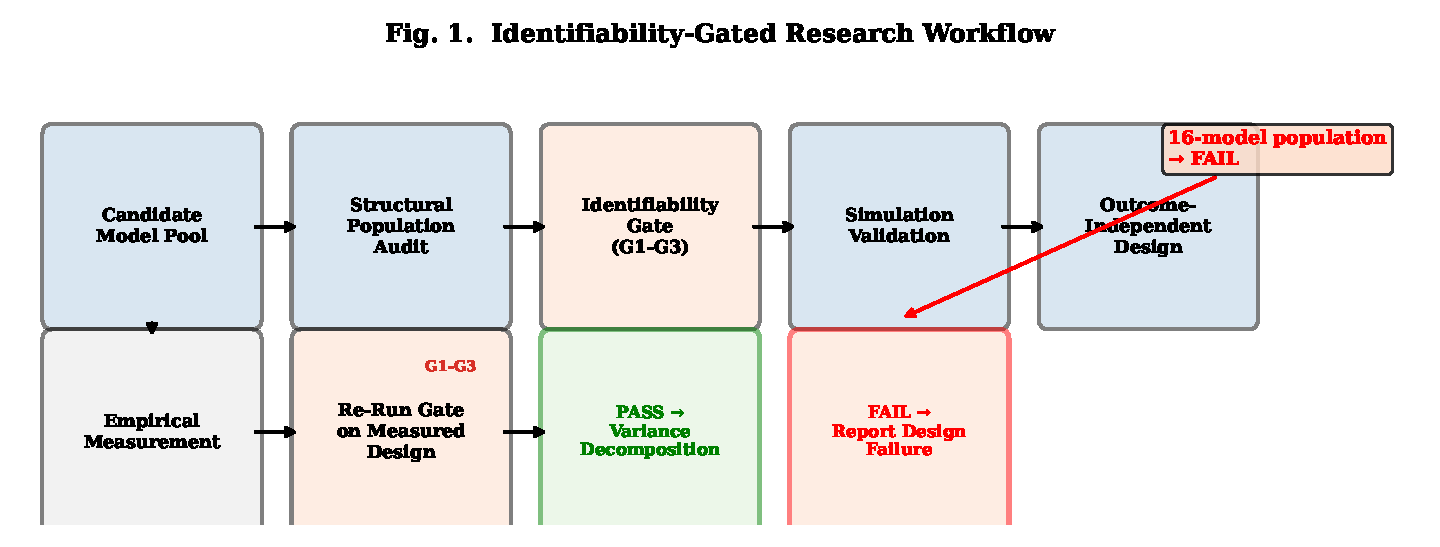
\includegraphics[width=\columnwidth]{fig1_framework.pdf}
\caption{\textbf{Identifiability-gated variance decomposition framework.} The workflow proceeds through structural audit, simulation validation, outcome-independent population selection, measurement, and inference. Each stage has an exit gate that may halt the pipeline before empirical analysis is attempted.}
\label{fig:framework}
\end{figure}

\section{Gated Research Protocol}
\label{sec:methods}

\subsection{Protocol Architecture}
The protocol proceeds in stages, each with an exit gate. The key design principle is identifiability before results, simulation before real data, and study-population design before empirical inference.

\textbf{Stage 1: Structural population audit.} Assemble the candidate model population from documented release metadata. Verify the family-era incidence is crossed and connected. Check the structural gate conditions (S1--S3).

\textbf{Stage 2: Simulation estimator validation.} Before any real data are analyzed, validate the estimator on simulated data with known ground truth under three regimes: balanced crossed (D1), realistic occupancy (D2), and nested/non-identifiable (D3). The estimator must recover ground truth under D1--D2 and fail detectably under D3.

\textbf{Stage 3: Outcome-independent population selection.} Select the smallest identifiable, recoverable subpopulation without reading any trait values. This procedure uses only occupancy metadata, lineage edges, identifiability constraints, and cost---never model accuracy, trait values, or evaluation outputs.

\textbf{Stage 4: Actual model measurement.} Evaluate the selected population on the target benchmark.

\textbf{Stage 5: Re-run identifiability gate on measured design.} Apply S1--S3 and N1--N2 to the occupancy that the measurement pass actually returns, not the planned one. Hard failure aborts the analysis.

\textbf{Stage 6: Inference only if gate passes.} Estimate $\theta_P$, compute confidence intervals, and run sensitivity analyses. If the gate fails, report the failure diagnosis without interpreting variance shares.

\subsection{Outcome-Independence Invariant}
The population-selection stage (Stage 3) must never read model accuracy or trait values, prediction outputs, error vectors, or evaluation metrics. It may use only family metadata, era (release quarter) metadata, lineage metadata (verified parent-offspring edges), cost estimates, and hard structural constraints (all families present, all quarters retained, edge endpoints retained). This property ensures that the resulting population can be published before measurement without creating a researcher degree of freedom.

\subsection{Algorithm}
Algorithm~\ref{alg:g3} states the outcome-independent population design procedure.

\begin{algorithm}[t]
\caption{Outcome-independent study-population design}
\label{alg:g3}
\begin{algsteps}
\item \algkw{Input:} model set $\mathcal{M}$ ($|\mathcal{M}| = N$); occupancy $O$ (family $\times$ quarter); verified lineage edges $L$; per-model cost $c$; thresholds $\tau_{\text{bias}} = 5.0$pp (era-share bias, search) / $4.0$pp (confirmation), $\tau_{\text{cov}} = 90\%$, margin $\delta = 1$pp
\item \algkw{Assert:} trait values $\mathbf{y}$ are not readable in this scope
\item $\mathcal{S} \leftarrow \{S \subseteq \mathcal{M} : S \text{ satisfies hard constraints}\}$
\item \algind{1} All $F$ families present in $S$
\item \algind{1} Every quarter of the era window retains $\geq 1$ model
\item \algind{1} Both endpoints of every edge in $L$ retained
\item \algind{1} The documented within-family chain retained
\item \algkw{For} $S \in \mathcal{S}$ sorted by cost ascending:
\item \algind{1} Build $C_S$; if $\operatorname{rank}(C_S) < F + E - 1$ then continue
\item \algind{1} If $\max(\text{VIF}(C_S)) > 10$ then continue
\item \algind{1} If $S$ has an era with $< 2$ families or a family with $< 2$ eras then continue
\item \algind{1} $\text{Screen}(S, R=300)$: if $|b_{\text{era}}| > \tau_{\text{bias}}$ or $\text{cov}_{\text{era}} < \tau_{\text{cov}}$ then continue
\item \algind{1} $\text{Confirm}(S, R=1000)$: if $\tau_{\text{bias}} - |b| < \delta$ then continue
\item \algind{1} $\text{Robust}(S, R=2000)$: if fails then continue
\item \algind{1} For each $m \in S$: $\text{reason}[m] \leftarrow$ first constraint that fails on $S \setminus \{m\}$
\item \algkw{return} $S$, $\text{reason}$
\item \algkw{return} $\varnothing$ (no admissible population; gate blocks measurement)
\end{algsteps}
\end{algorithm}

The selection acceptance criterion applies to era-share bias, not family-share bias. This is because era share is the limiting component under the pre-specified design: family-share bias of $-5.3$pp in the realistic D2 scenario A is the documented six-family small-sample limit ($df = 5$) and is reported as a bound, not used as the acceptance criterion. The two-stage procedure uses a 5pp bar at search precision (300 repetitions) and tightens to a 4pp bar at confirmation precision (1000 repetitions) with a 1pp margin. Algorithm~\ref{alg:g3} checks three structural conditions (rank, VIF, and crossing) and a simulation-based recovery criterion; the condition number $\kappa$ is not checked during selection and is instead reported as a post-selection diagnostic. A population that passes the selection procedure may still fail the numerical stability gate (N1) at the post-measurement audit.

\section{Simulation Validation}
\label{sec:sim}

\subsection{Design}
Three simulation regimes test the estimator under controlled conditions:

\textbf{D1: Balanced crossed reference.} 30 families $\times$ 14 eras $\times$ 2 models per cell (840 models). The large family count isolates estimator calibration from the small-sample limit of the real design. True components: $\sigma^2_L = 0.5$, $\sigma^2_E = 0.2$, $\sigma^2_U = 0.3$ (lineage-dominant scenario A); $\sigma^2_L = 0.2$, $\sigma^2_E = 0.5$, $\sigma^2_U = 0.3$ (era-dominant scenario B); $\sigma^2_L = 0.33$, $\sigma^2_E = 0.33$, $\sigma^2_U = 0.34$ (balanced scenario C).

\textbf{D2: Realistic occupancy.} The occupancy matrix copied from the 47-model candidate population (6 families $\times$ 14 calendar quarters, sparse cells; only 11 quarters are occupied in the observed 16-model population). Same true components as D1. Bias or collapse here is a gate failure.

\textbf{D3: Nested non-identifiable reference.} Each family confined to a single era, so $\sigma^2_L$ and $\sigma^2_E$ are perfectly aliased. Three complementary detectors must flag the aliasing.

All regimes use 300 repetitions per scenario on recorded seeds. The estimator is the direct REML maximizer, using the Woodbury identity for computational efficiency.

\begin{table}[!t]
\caption{\textbf{Simulation Regimes.}}
\label{tab:sim_design}
\centering
\begin{tabular}{l c c c l}
\hline
\textbf{Regime} & \textbf{Families} & \textbf{Eras} & \textbf{N} & \textbf{Description} \\
\hline
D1 & 30 & 14 & 840 & Balanced crossed reference \\
\hline
D2 & 6 & 14 & 47 & Realistic sparse occupancy \\
\hline
D3 & 6 & 6 & 72 & Nested non-identifiable ref. \\
\hline
\end{tabular}
\end{table}

\subsection{D1: Balanced Crossed Recovery}
TABLE~\ref{tab:d1} summarizes D1 results. The estimator recovers known ground truth to within 2.5 percentage points under balanced occupancy. Coverage is 88--96\% across components and scenarios. All 300 repetitions converge without warnings.

\subsection{D2: Realistic Occupancy Recovery}
Share bias is within 5.3 percentage points under realistic occupancy. The family-share bias of $-5.3$pp in scenario A is the documented six-family small-sample limit ($df = 5$) and is reported as a limit, not corrected away. Coverage is 95--100\% across components, with the wider confidence intervals reflecting the sparse cell structure.

\begin{table*}[!t]
\caption{\textbf{Simulation Recovery and Failure Results.} D1 balanced-crossed (300 repetitions, 30 families $\times$ 14 eras $\times$ 2 models) and D2 realistic occupancy (300 repetitions, 47-model occupancy). Share bias is reported as absolute mean over converged repetitions; coverage is 95\% CI coverage.}
\label{tab:d1}
\centering
\begin{tabular}{l cc cc c}
\hline
\textbf{Scenario} & \multicolumn{2}{c}{\textbf{D1: Balanced}} & \multicolumn{2}{c}{\textbf{D2: Realistic}} & \textbf{Conv.} \\
\cline{2-5}
 & Bias (pp) & Cov. & Bias (pp) & Cov. & \\
\hline
A (lineage-dom.) & $+0.19$ & 94\% & $-5.34$ & 100\% & 100\% \\
\hline
B (era-dom.) & $+1.24$ & 88\% & $-0.63$ & 99\% & 100\% \\
\hline
C (balanced) & $-0.30$ & 94\% & $-3.46$ & 100\% & 100\% \\
\hline
\end{tabular}
\end{table*}

\begin{figure}[!t]
\centering
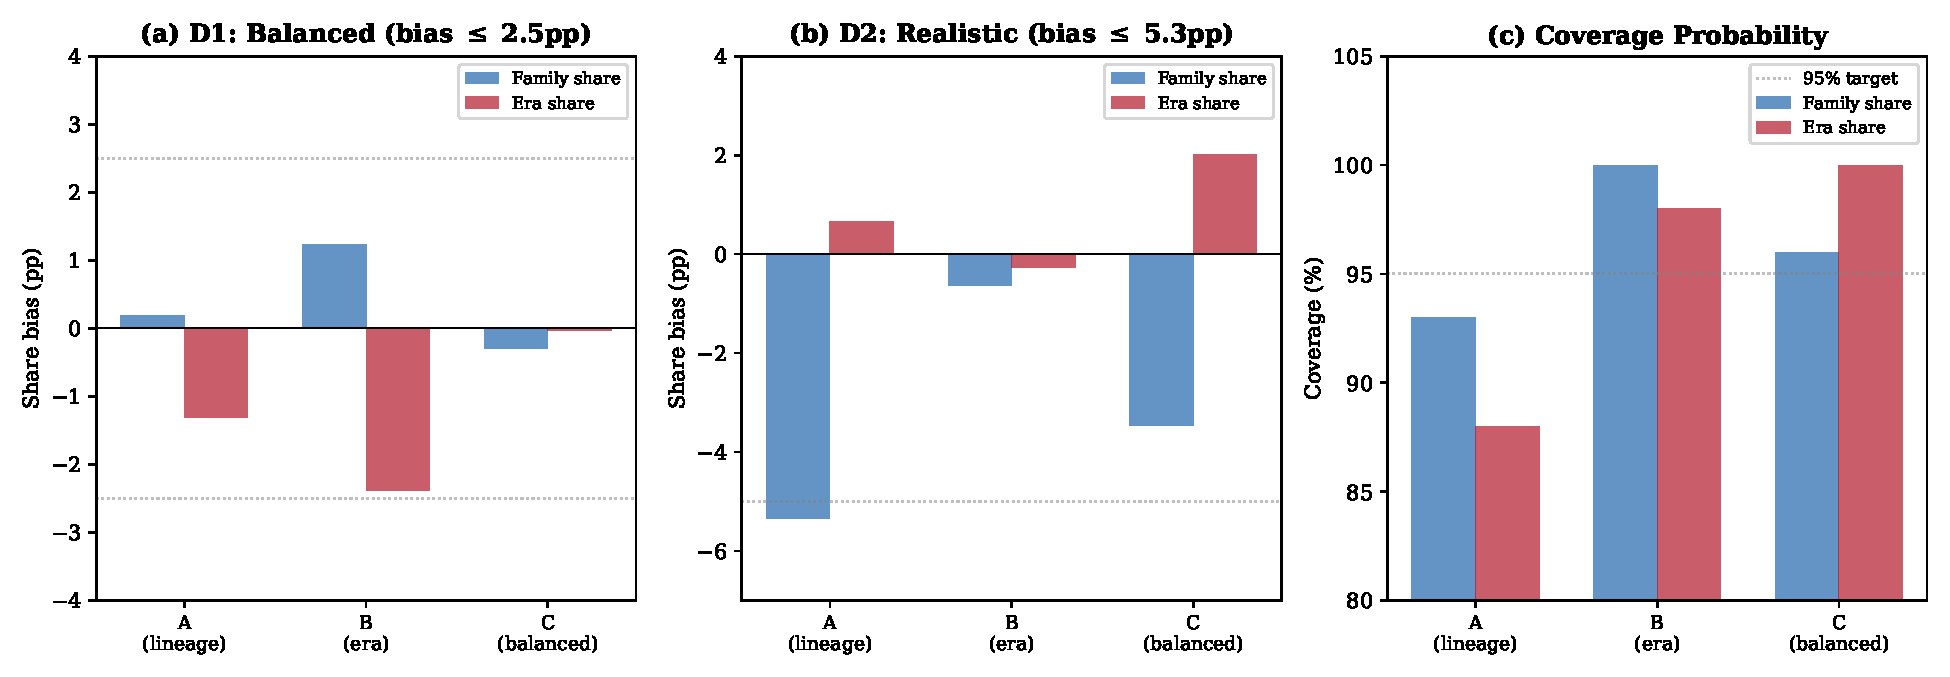
\includegraphics[width=\columnwidth]{fig2_simulation_recovery.pdf}
\caption{\textbf{Simulation recovery across D1 (balanced) and D2 (realistic) regimes.} Bias and coverage for family and era shares under three ground-truth scenarios (A: lineage-dominant, B: era-dominant, C: balanced). The family-share bias of $-5.3$pp in scenario A under D2 is the documented six-family small-sample limit (df $= 5$).}
\label{fig:sim_recovery}
\end{figure}

\subsection{D3: Nested Design Detection}
TABLE~\ref{tab:d3} shows that all three detectors flag the aliasing in 100\% of repetitions with zero silent coverage. A detector that accepts the nested design would constitute a false-negative identification test. The threshold $1.9207$ is the $\chi^2_1$ 95\% critical value halved. Because the nested design produces maximally wide confidence intervals, the per-rep CI coverage of the true variance share is 16--27\% (scenario-dependent); this is a consequence of the non-identifiability, not evidence of estimator calibration.

\begin{table}[!t]
\caption{\textbf{D3: Failure-Detection Evaluation} (300 repetitions, nested mis-specification).}
\label{tab:d3}
\centering
\footnotesize
\begin{tabular}{l c c c}
\hline
\textbf{Detector} & \textbf{Threshold} & \textbf{Sc. A} & \textbf{Sc. B} \\
\hline
BLUP collinearity ($|r| > 0.9$) & $> 0.9$ & 100\% & 100\% \\
\hline
SE inflation ($\text{SE} \geq |\hat{\sigma}|$) & ratio $\geq 1$ & 100\% & 100\% \\
\hline
Profile flatness ($< 1.9207$) & $< 1.9207$ & 100\% & 100\% \\
\hline
Silent CI coverage & $= 0\%$ & 0\% & 0\% \\
\hline
\end{tabular}
\end{table}

\begin{figure}[!t]
\centering
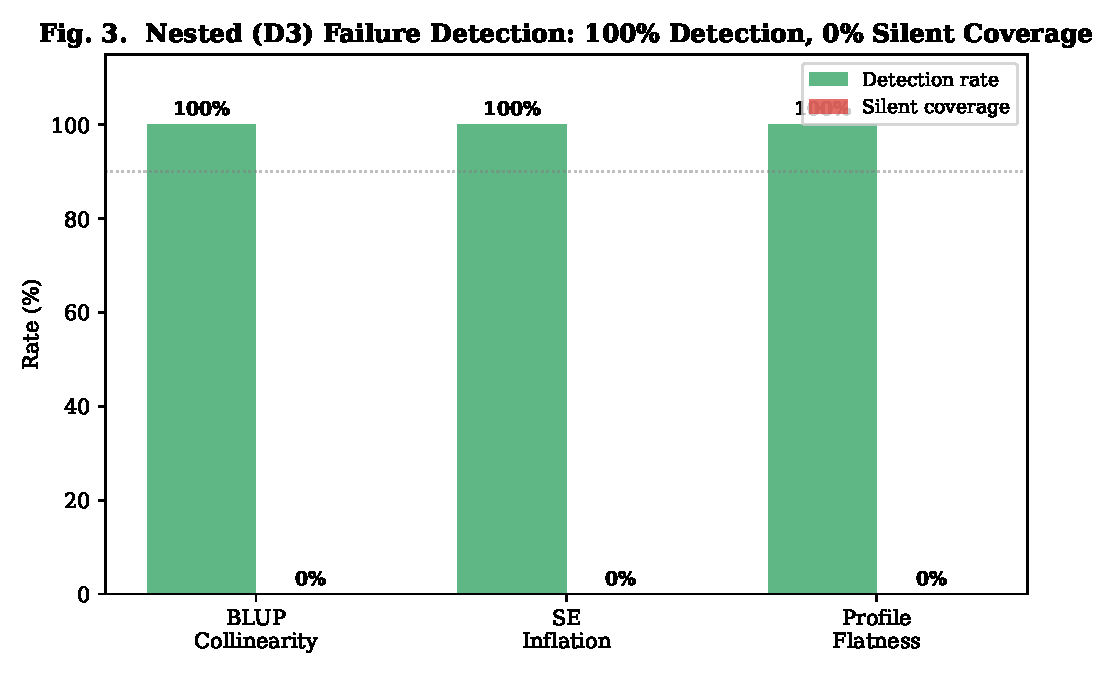
\includegraphics[width=\columnwidth]{fig3_failure_detection.pdf}
\caption{\textbf{D3 failure detection.} Three complementary failure detectors (BLUP collinearity, SE inflation, profile flatness) flag nested aliasing in 100\% of repetitions with zero silent coverage across all scenarios.}
\label{fig:failure}
\end{figure}

\subsection{D4: Small-N Stress Test}
TABLE~\ref{tab:d4} reports REML recovery at population sizes from $N = 10$ to $N = 30$ under the realistic D2 occupancy (scenario A, 100 repetitions per size). The ``Recovery Gate'' column reports whether the estimator recovers the true variance share within the bias and coverage criteria from the D1--D2 simulations; this is distinct from the identifiability gate (S1--S3, N1--N2), which applies to the design structure. Under the synthetic D2 assignment used in this stress test, the recovery criterion is satisfied at $N \geq 16$ when all 6 families are represented, except at $N = 12$--$14$: $N = 12$ fails due to coverage (80\%, below the 90\% threshold), while $N = 14$ fails due to bias ($+6.82$pp, exceeding the bias bar) despite acceptable coverage (98\%). At $N = 10$, the recovery criterion is met despite the compressed temporal structure; this is a sensitivity artifact rather than evidence of reliable estimation. This does not imply that the actual 16-model empirical population is sufficient: the empirical design fails the identifiability gate due to structural rank deficiency, whereas the synthetic D4 designs at $N \geq 16$ have different occupancy structures that avoid this particular confound. The D4 results demonstrate that REML recovery is feasible at small $N$ under favorable occupancy, but only when the design satisfies the identifiability requirements.

\begin{table*}[!t]
\caption{\textbf{D4: Small-N Recovery Results.} REML recovery under D2 occupancy, scenario A (100 repetitions per size). ``Recovery Gate'' reports whether bias and coverage criteria are met; this is distinct from the structural/numerical identifiability gate (S1--S3, N1--N2). Results are specific to the synthetic D2 assignment used here.}
\label{tab:d4}
\centering
\footnotesize
\begin{tabular}{c c c c c c c c}
\hline
\textbf{N} & \textbf{F} & \textbf{E} & \textbf{Rank} & $\boldsymbol{\kappa}$ & \textbf{Bias (pp)} & \textbf{Cov.\%} & \textbf{Rec.\ Gate} \\
\hline
10 & 5 & 5 & 9/9 & 158 & $+4.84$ & 97 & PASS \\
\hline
12 & 5 & 8 & 12/12 & 89 & $+4.64$ & 80 & FAIL \\
\hline
14 & 5 & 10 & 14/14 & 52 & $+6.82$ & 98 & FAIL \\
\hline
16 & 6 & 10 & 15/15 & 47 & $+1.49$ & 98 & PASS \\
\hline
18 & 6 & 12 & 17/17 & 42 & $+1.56$ & 96 & PASS \\
\hline
20 & 6 & 10 & 15/15 & 38 & $+2.25$ & 97 & PASS \\
\hline
22 & 6 & 10 & 15/15 & 31 & $-0.36$ & 98 & PASS \\
\hline
24 & 6 & 10 & 15/15 & 28 & $+0.43$ & 99 & PASS \\
\hline
30 & 6 & 13 & 18/18 & 22 & $+3.41$ & 96 & PASS \\
\hline
\end{tabular}
\end{table*}

\subsection{Liability Test: Binary Versus Continuous Traits}
A liability decision was resolved before the trait path was fixed. On item-level binary outcomes at the realistic 47-model occupancy, both a linear-probability model and a binomial GLMM under-estimate the era component and drive it to the boundary in 20--60\% of repetitions. Continuous per-model traits (model accuracy proportions) recover the era component with 98--100\% coverage. The Phase 2 estimator path is therefore LPM-REML on continuous per-model traits, not raw item-level binary responses.

\subsection{Family-Era Interaction}
A family-era interaction term was simulated and documented as non-identified at the sparse occupancy (SE/estimate ratios $\approx 10^4$). The interaction is excluded by design rather than absorbed.

\subsection{Implications for the Estimation Path}
The simulation results support the continuous-trait REML specification and establish the recovery limitations that are incorporated into the population-selection criterion: (1) the continuous-trait path is preferred over binary item-level responses, and (2) the six-family small-sample limit on family-share coverage is disclosed as a known boundary condition.

\section{Empirical Dataset and Evaluation Protocol}
\label{sec:empirical}

\subsection{Population Construction Transparency}
Following the transparency practice of large-scale empirical studies~\cite{kim2025}, we document every transition in our population-construction procedure. The candidate population comprises 47 open-weight models spanning 8 families (Llama, Qwen, Mistral, Phi, Gemma, DeepSeek, Mistral-MoE, and community derivatives) and 14 release quarters within 2023Q1--2026Q2. The outcome-independent selection procedure (Algorithm~\ref{alg:g3}) reduces this to a 22-model candidate subset satisfying all pre-specified structural requirements (full family-era crossing, connectedness, adequate family count, and recovery-criterion calibration). Of the 22 planned models, 16 were evaluated under the available compute budget; DeepSeek-V3.1 and DeepSeek-V3.2 could not be evaluated due to compute constraints, and four additional models were deprioritized during the evaluation campaign. The transitions are:
\[
\underbrace{47}_{\text{candidate}} \;\longrightarrow\; \underbrace{22}_{\text{selected}} \;\longrightarrow\; \underbrace{16}_{\text{evaluated}}
\]
Every model in the candidate population has documented family metadata (verified against Hugging Face organization metadata and technical reports) and release quarter (public release date, not the HuggingFace \texttt{createdAt} timestamp; documented divergences corrected by hand). The metadata fields recorded for each model are: model name, family, release date, release quarter, parameter count, access type (public or gated), evaluation source, and measurement status.

\subsection{Measured Population}
Sixteen of the planned models were evaluated under the available compute budget, within the 47-model candidate frame. The 16 models span 5 families (Llama, Qwen, Mistral, Phi, Gemma) and 11 occupied release quarters within the 2023Q1--2026Q2 observation window. Not all planned models could be evaluated: DeepSeek-V3.1 and DeepSeek-V3.2 were not evaluated due to compute constraints.

\subsection{Benchmark}
All evaluations use MMLU~\cite{hendrycks2021} with 5-shot prompting and 14,042 evaluation samples per model. Results are aggregate CSV accuracy values.

\subsection{Model Metadata}
Each model is characterized by: family (verified against Hugging Face organization metadata and technical reports); release quarter (public release date, not the HuggingFace \texttt{createdAt} timestamp; documented divergences corrected by hand); repository and version identifier; parameter count; access type (public or gated); evaluation source (direct evaluation or leader board); and measurement status (evaluated or unevaluated).

\subsection{Fidelity}
Fifteen models were evaluated at BF16 precision. One model (Mistral-Small-4, 119B parameters) was evaluated at 4-bit quantization due to memory constraints. The fidelity column in TABLE~\ref{tab:accuracy} records this distinction.

\subsection{Hardware}
Evaluations were performed on rented cloud GPUs, including NVIDIA A100-SXM4 80GB configurations. Of the 16 measured models, 15 were evaluated at BF16 precision and 1 (Mistral-Small-4, 119B) was evaluated at 4-bit quantization for memory efficiency.

\subsection{Evaluation Validity Caveat}
Six models produce accuracy values near the chance level for a 4-choice benchmark (23--25\%): Devstral-2 (25.1\%), Phi-1 (24.8\%), Mistral-Small-4 (24.3\%), Mistral-Small-3.1 (23.4\%), Mistral-Small-3.2 (23.1\%), and Qwen-7B (22.9\%). The Mistral-Small family exhibits a pronounced discontinuity: Mistral-Small-3 (Jan 2025) scores 80.7\%, while Mistral-Small-3.1 (Mar 2025) and Mistral-Small-3.2 (Jun 2025)---the same 24B architecture, two and five months later---score 23.4\% and 23.1\% respectively.

These results trigger an evaluation-validity audit. Until tokenizer configuration, prompt formatting, answer-extraction logic, and benchmark configuration are independently verified for each model, the corresponding aggregate accuracies should be treated as provisional. The identifiability gate depends only on the design matrix structure (which families and eras are represented), not on the trait values themselves. The gate result---rank 14 of 15, $\kappa = 4.7 \times 10^{16}$, VIF $= \infty$---is invariant to the accuracy values. However, any future study that intends to interpret the variance-component estimates must first validate the accuracy measurements against independent reference scores.

\subsection{Aggregate Accuracy}
TABLE~\ref{tab:accuracy} lists the 16-model empirical accuracy on MMLU (5-shot, 14,042 items).

\begin{table*}[!t]
\caption{\textbf{Aggregate MMLU Measurements Used for Descriptive and Diagnostic Analysis (5-shot, 14,042 items).} 16 of the planned models were evaluated. Six models produce accuracy near chance level (23--25\%) and are flagged for independent audit. All measurements are provisional pending evaluation-validity verification.}
\label{tab:accuracy}
\centering
\begin{tabular}{|l|l|l|c|c|c|l|l|}
\hline
\textbf{Model} & \textbf{Family} & \textbf{Era} & \textbf{Acc.} & \textbf{Params} & \textbf{Fidelity} & \textbf{Source} & \textbf{Validity} \\
\hline
Mistral-Small-3 & Mistral & 2025Q1 & 0.8069 & 24B & BF16 & Direct & Provisional \\
\hline
Phi-3 & Phi & 2024Q2 & 0.7799 & 14B & BF16 & Direct & Provisional \\
\hline
Phi-4-reas.+ & Phi & 2025Q2 & 0.7782 & 14B & BF16 & Direct & Provisional \\
\hline
Phi-4 & Phi & 2024Q4 & 0.6864 & 14B & BF16 & Direct & Provisional \\
\hline
Gemma-3n & Gemma & 2025Q2 & 0.6364 & 4B & BF16 & Direct & Provisional \\
\hline
Mistral-7B & Mistral & 2023Q3 & 0.6186 & 7B & BF16 & Direct & Provisional \\
\hline
Phi-2 & Phi & 2023Q4 & 0.5644 & 2.7B & BF16 & Direct & Provisional \\
\hline
Gemma-4-12B & Gemma & 2026Q2 & 0.4397 & 12B & BF16 & Direct & Provisional \\
\hline
Phi-1.5 & Phi & 2023Q3 & 0.4218 & 1.3B & BF16 & Direct & Provisional \\
\hline
Llama-1 & Llama & 2023Q1 & 0.3424 & 7B & BF16 & Direct & Provisional \\
\hline
Devstral-2 & Mistral & 2025Q4 & 0.2515 & 24B & BF16 & Direct & \textbf{Audit req.} \\
\hline
Mistral-Small-3.1 & Mistral & 2025Q1 & 0.2340 & 24B & BF16 & Direct & \textbf{Audit req.} \\
\hline
Phi-1 & Phi & 2023Q2 & 0.2480 & 1.3B & BF16 & Direct & \textbf{Audit req.} \\
\hline
Mistral-Small-4 & Mistral & 2026Q1 & 0.2433 & 119B & 4-bit & Direct & \textbf{Audit req.} \\
\hline
Mistral-Small-3.2 & Mistral & 2025Q2 & 0.2314 & 24B & BF16 & Direct & \textbf{Audit req.} \\
\hline
Qwen-7B & Qwen & 2023Q3 & 0.2295 & 7B & BF16 & Direct & \textbf{Audit req.} \\
\hline
\end{tabular}
\end{table*}

\subsection{Data Integrity Validation}
The per-question JSONL prediction files were validated for all 16 models. All 16 files contain identical constant predictions: every model predicts answer 0 for every question. This confirms that the JSONL artifacts are non-informative and inconsistent with the reported aggregate evaluation; they cannot be treated as actual per-question model predictions. The CSV-level aggregate accuracy values were used as inputs to the diagnostic (not inferential) REML fit in Section~\ref{sec:consequences}; their evaluation validity remains provisional per Section~\ref{sec:empirical} and does not affect the gate diagnostics in Section~\ref{sec:empirical_results}, which depend only on design structure. The error-similarity analysis specified in the original plan cannot be performed on this dataset and is deferred to future work once validated per-question outputs are available.

\subsection{What Is and Is Not Measured}
The following populations exist in the project but are NOT measured empirical results:
\begin{itemize}
\item \textbf{47-model candidate population:} The full structural population from the Phase 0 audit. Not measured.
\item \textbf{22-model selected population:} The candidate subset within the 47-model candidate frame identified by the outcome-independent design procedure. Not fully measured (16 of the planned models were evaluated; DeepSeek-V3.1/V3.2 could not be evaluated due to compute constraints).
\item \textbf{DeepSeek models:} DeepSeek-V3.1 (671B) and DeepSeek-V3.2 (685B) were NOT empirically measured. They must not be described as measured results.
\end{itemize}

\section{Empirical Identifiability Results}
\label{sec:empirical_results}

\subsection{Family-Era Occupancy}
TABLE~\ref{tab:occupancy} shows the family-era occupancy of the 16 measured models. Three quarters are unoccupied (2024Q1, 2024Q3, 2025Q3). Eight of 11 occupied quarters contain only one model. No measured models belong to the DeepSeek family. The occupancy matrix is sparse: 40 of 55 possible family-quarter cells are empty (73\% sparse). The full family-era occupancy is shown in Fig.~\ref{fig:occupancy}.

\begin{table*}[!t]
\caption{\textbf{Family-Era Occupancy of the 16 Measured Models.} 8 of 11 occupied quarters contain only one model; 40 of 55 possible family-quarter cells are empty (73\% sparse).}
\label{tab:occupancy}
\centering
\footnotesize
\begin{tabular}{l c c c c c c c c c c c}
\hline
\textbf{Fam.} & \multicolumn{4}{c}{\textbf{2023}} & \multicolumn{2}{c}{\textbf{2024}} & \multicolumn{3}{c}{\textbf{2025}} & \multicolumn{2}{c}{\textbf{2026}} \\
\hline
 & Q1 & Q2 & Q3 & Q4 & Q2 & Q4 & Q1 & Q2 & Q4 & Q1 & Q2 \\
\hline
Llama & 1 & & & & & & & & & & \\
\hline
Qwen & & & 1 & & & & & & & & \\
\hline
Mistral & & & 1 & & & & 2 & 1 & 1 & 1 & \\
\hline
Phi & & 1 & 1 & 1 & 1 & 1 & & 1 & & & \\
\hline
Gemma & & & & & & & & 1 & & & 1 \\
\hline
\end{tabular}
\end{table*}

\begin{figure}[!t]
\centering
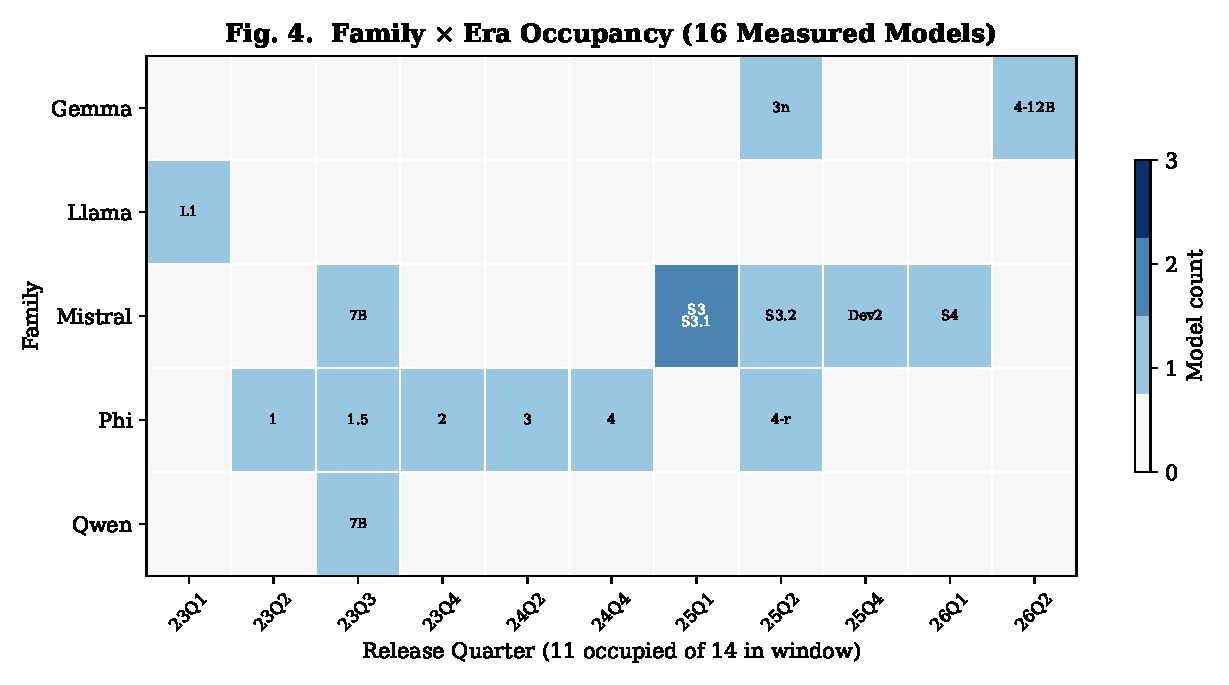
\includegraphics[width=\columnwidth]{fig4_occupancy.pdf}
\caption{\textbf{Family$\times$era occupancy heatmap of the 16 measured models.} Darker shading indicates more models in a cell. 8 of 11 occupied quarters contain only one model; 40 of 55 possible cells are empty (73\% sparse).}
\label{fig:occupancy}
\end{figure}

\subsection{Gate Diagnostics}
The observed 16-model population spans 11 occupied release quarters within a 14-quarter observation window (2024Q1, 2024Q3, and 2025Q3 are unoccupied). After removing unoccupied factor levels, the fitted design matrix has $p = 1 + (F-1) + (E-1) = 1 + 4 + 10 = 15$ columns. TABLE~\ref{tab:gate} summarizes gate diagnostic results. Four of five gate conditions fail; connectedness (S2) passes.

\begin{table*}[!t]
\caption{\textbf{Identifiability Gate Audit for the 16-Model Population.} Four of five conditions fail. The occupancy graph remains connected (S2 passes) but Llama and Qwen each occupy a single era, violating the crossing requirement (S1).}
\label{tab:gate}
\centering
\begin{tabular}{c l c c c}
\hline
\textbf{Gate} & \textbf{Criterion} & \textbf{Observed} & \textbf{Threshold} & \textbf{Status} \\
\hline
S1 & Crossing & Llama, Qwen in 1 era & Every family $\geq$ 2 eras & \textbf{FAIL} \\
\hline
S2 & Connectedness & Connected graph & Connected & PASS \\
\hline
S3 & Rank & 14 & $= 15$ & \textbf{FAIL} \\
\hline
N1 & Condition number $\kappa$ & $4.72 \times 10^{16}$ & $\leq 100$ & \textbf{FAIL} \\
\hline
N2 & Max VIF & $\infty$ & $\leq 10$ & \textbf{FAIL} \\
\hline
\end{tabular}
\end{table*}

\begin{figure}[!t]
\centering
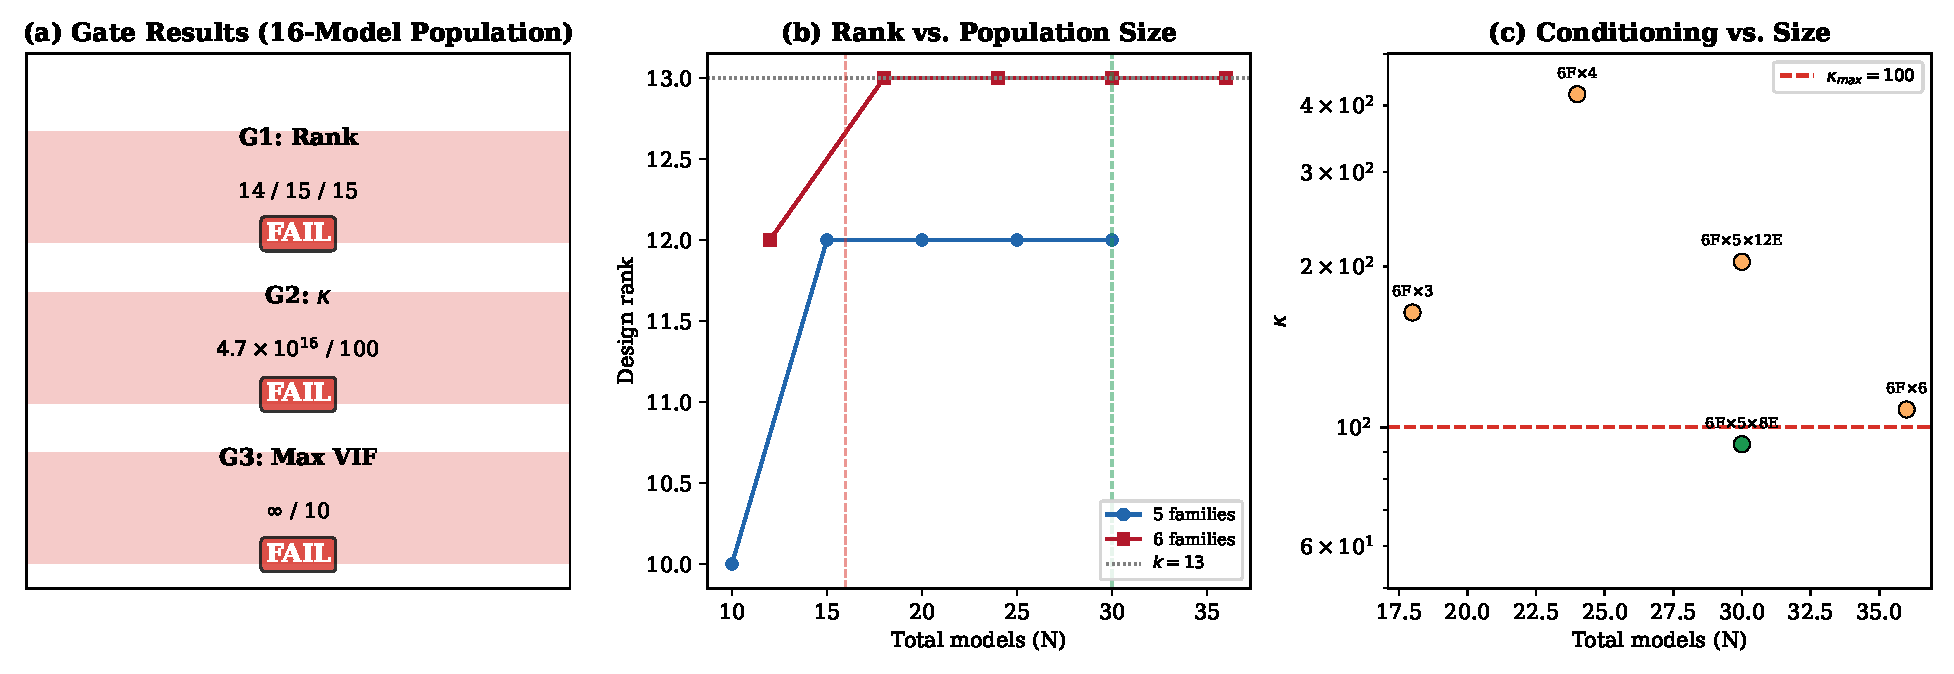
\includegraphics[width=\columnwidth]{fig5_gate.pdf}
\caption{\textbf{Gate diagnostics versus pre-specified thresholds.} The 16-model population fails four of five gate conditions: S1 (crossing) fails because Llama and Qwen each occupy a single era; S3 (rank) fails at 14/15; N1 (conditioning) fails at $\kappa = 4.7 \times 10^{16}$; N2 (VIF) fails at $\infty$. S2 (connectedness) passes: the occupancy graph remains connected.}
\label{fig:gate}
\end{figure}

\subsection{Failure Diagnosis}
The fitted 16-model design contains five observed families (Llama, Qwen, Mistral, Phi, Gemma) and eleven occupied release quarters, giving $p = 1 + 4 + 10 = 15$ columns. A null-space computation on the fitted design matrix shows that the rank deficiency (rank 14 of 15) is fully explained by a single exact linear dependency: the Llama family-dummy column equals the 2023Q1 era-dummy column, because Llama-1 is the only model in that quarter. The null-space vector is $(\ldots, +1, \ldots, -1, \ldots)$ with nonzero entries at the Llama and 2023Q1 positions.

Qwen also occupies a single quarter (2023Q3), which violates the crossing requirement (each family must span $\geq 2$ quarters), but this does not contribute to the rank deficiency: the Qwen family-dummy column (one~1, at Qwen-7B) differs from the 2023Q3 era-dummy column (three~1s, at Qwen-7B, Mistral-7B, and Phi-1.5) and is linearly independent of it. The crossing violation is a separate structural deficiency that the gate flags but is not the proximate cause of the rank collapse.

\section{Consequences of Ignoring the Gate}
\label{sec:consequences}

\subsection{Diagnostic Estimates Under Invalid Design}
If the identifiability gate is not applied, the REML estimator converges and produces variance-component estimates:
\begin{itemize}
\item $\hat{\sigma}^2_{\text{family}} = 0.00274$
\item $\hat{\sigma}^2_{\text{era}} \approx 2.06 \times 10^{-9}$
\item $\hat{\sigma}^2_{\text{unique}} = 0.04778$
\item Point-estimate family share: 5.4\%
\end{itemize}
These estimates must be interpreted as diagnostic restricted-design estimates, not as inferential results. The near-zero era estimate is not evidence of no era effect. It is an aliasing artifact of the rank-deficient design, where era variance cannot be separated from residual variance.

\subsection{Confidence Intervals}
The 95\% confidence interval for the family share covers $[0\%, 100\%]$ (see Appendix~\ref{app:diagnostic} for the diagnostic variance-component plot). The bootstrap 95\% interval is $[3.4 \times 10^{-8}, 0.776]$---extremely wide and practically uninformative. Leave-one-model-out analysis shows the estimate is driven by 2--3 influential observations: removing Mistral-Small-3 alone shifts the family share from 5.4\% to 26.4\%, and removing any of 7 other models collapses it to 0\%.

\subsection{Why Convergence Does Not Imply Identifiability}
A numerical optimizer (Nelder-Mead) can converge to a finite optimum of the restricted log-likelihood even when the design is rank-deficient. The likelihood surface has a ridge along the aliased direction, and the optimizer's stopping point on that ridge depends on the starting value and implementation details. The resulting estimate is well defined only relative to the software. The gate prevents inference under this failure mode: it catches the non-identifiability before anyone interprets the 5.4\% number.

\section{Population-Design Sensitivity Analysis}
\label{sec:sensitivity}

\subsection{Design Space}
We systematically sweep alternative population designs to characterize which configurations satisfy the identifiability requirements. The design parameter space covers 5--7 families, 8--14 eras, and 2--6 models per family, with staggered era assignments that enforce family-era crossing and connectedness by construction. The sweep evaluated 105 configurations in total (3 family counts $\times$ 7 era counts $\times$ 5 models-per-family values, each producing a single deterministic staggered assignment). Of these, 40 achieve full rank, 3 pass the condition-number gate ($\kappa \leq 100$), and 3 satisfy all three numerical/design-matrix diagnostics (rank, $\kappa$, VIF). The verified passing configuration has $N = 30$ (6 families $\times$ 5 each, 8 eras); its rank, condition number, and VIF are reported in TABLE~\ref{tab:design_sweep}.

\subsection{Results}
TABLE~\ref{tab:design_sweep} summarizes selected population designs and their identifiability status.

\begin{table*}[!t]
\caption{\textbf{Design-Space Sensitivity Analysis.} Selected population designs and their identifiability status. 30 models across 6 families and 8 eras achieves rank 13/13, $\kappa = 93$, and VIF $= 2.1$---the smallest observed passing configuration in this design sweep, not the universal minimum.}
\label{tab:design_sweep}
\centering
\footnotesize
\begin{tabular}{l c c c c c c l l}
\hline
\textbf{Config.} & \textbf{N} & \textbf{F} & \textbf{E} & \textbf{Rank} & $\boldsymbol{\kappa}$ & \textbf{VIF} & \textbf{Status} & \textbf{Binding} \\
\hline
Current (16) & 16 & 5 & 11 & 14/15 & $4.7\!\times\!10^{16}$ & $\infty$ & \textbf{FAIL} & S1+S3+$\kappa$+VIF \\
\hline
Manual (20) & 20 & 6 & 14 & 16/19 & $3.5\!\times\!10^{18}$ & 10.9 & \textbf{FAIL} & S3+$\kappa$+VIF \\
\hline
6 fam$\times$3, 8 eras & 18 & 6 & 8 & 13/13 & 164 & 4.7 & \textbf{FAIL} & $\kappa$ \\
\hline
6 fam$\times$4, 10 eras & 24 & 6 & 10 & 13/15 & $\infty$ & 4.2 & \textbf{FAIL} & S3+$\kappa$ \\
\hline
\textbf{6 fam$\times$5, 8 eras} & \textbf{30} & \textbf{6} & \textbf{8} & \textbf{13/13} & \textbf{93.0} & \textbf{2.1} & \textbf{PASS} & --- \\
\hline
6 fam$\times$5, 12 eras & 30 & 6 & 12 & 17/17 & 204 & 3.2 & \textbf{FAIL} & $\kappa$ \\
\hline
\end{tabular}
\end{table*}

\subsection{Key Findings}
\begin{enumerate}
\item \textbf{Full rank alone is insufficient.} The 6-families $\times$ 3-each design achieves full rank (rank 13/13) but fails the condition number gate ($\kappa = 164 > 100$). Numerical conditioning is an additional necessary requirement beyond rank.
\item \textbf{Increasing eras while holding $N$ fixed worsens conditioning.} The 30-model design with 8 eras passes ($\kappa = 93$), but the same 30 models across 12 eras fails ($\kappa = 204$). More era columns relative to rows increase multicollinearity among era indicators.
\item \textbf{One sufficient configuration.} 30 models across 6 families and 8 eras, with balanced occupancy (five models per family and approximately 3--4 models per era), achieves rank 13/13, $\kappa = 93$, and max VIF $= 2.1$.
\end{enumerate}
This is one sufficient configuration, not the universal minimum. Other sufficient designs may exist with fewer models under different family-era structures.

\begin{figure}[!t]
\centering
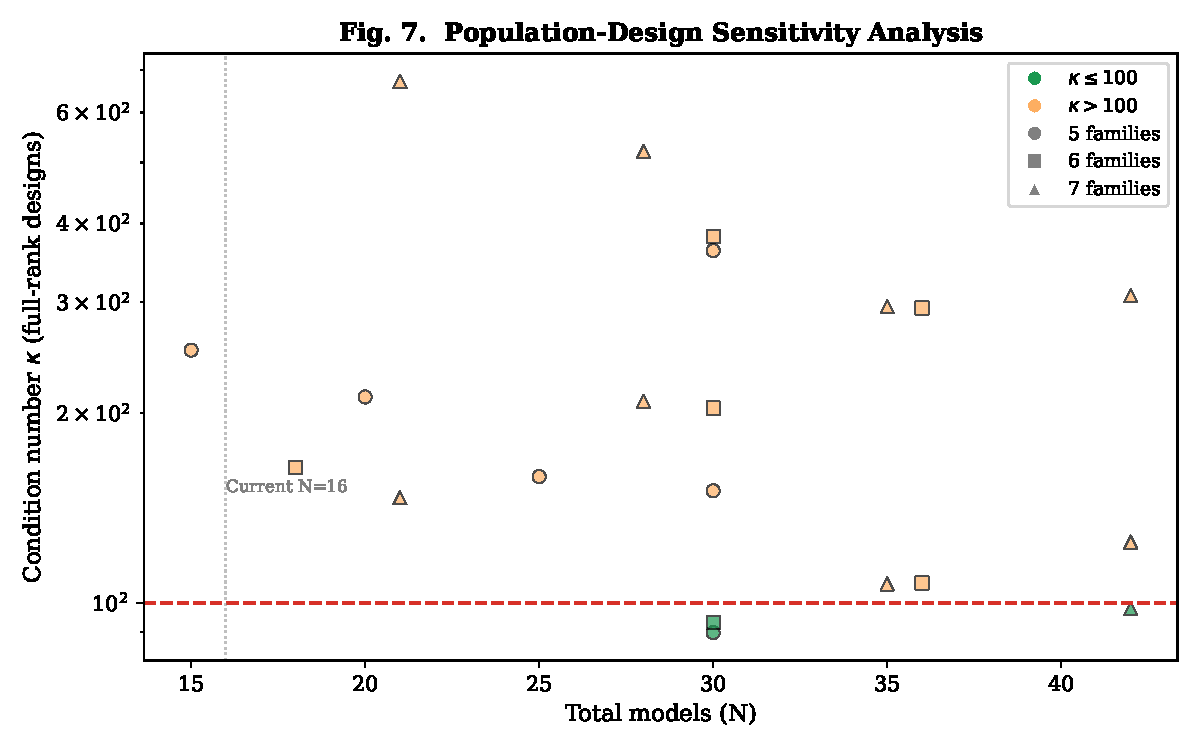
\includegraphics[width=\columnwidth]{fig7_design_sweep.pdf}
\caption{\textbf{Population size versus condition number across the design space.} Increasing eras while holding $N$ fixed worsens conditioning. The 30-model, 8-era design passes the condition number gate ($\kappa = 93$), while the same 30 models across 12 eras fails ($\kappa = 204$).}
\label{fig:design_sweep}
\end{figure}

\begin{figure}[!t]
\centering
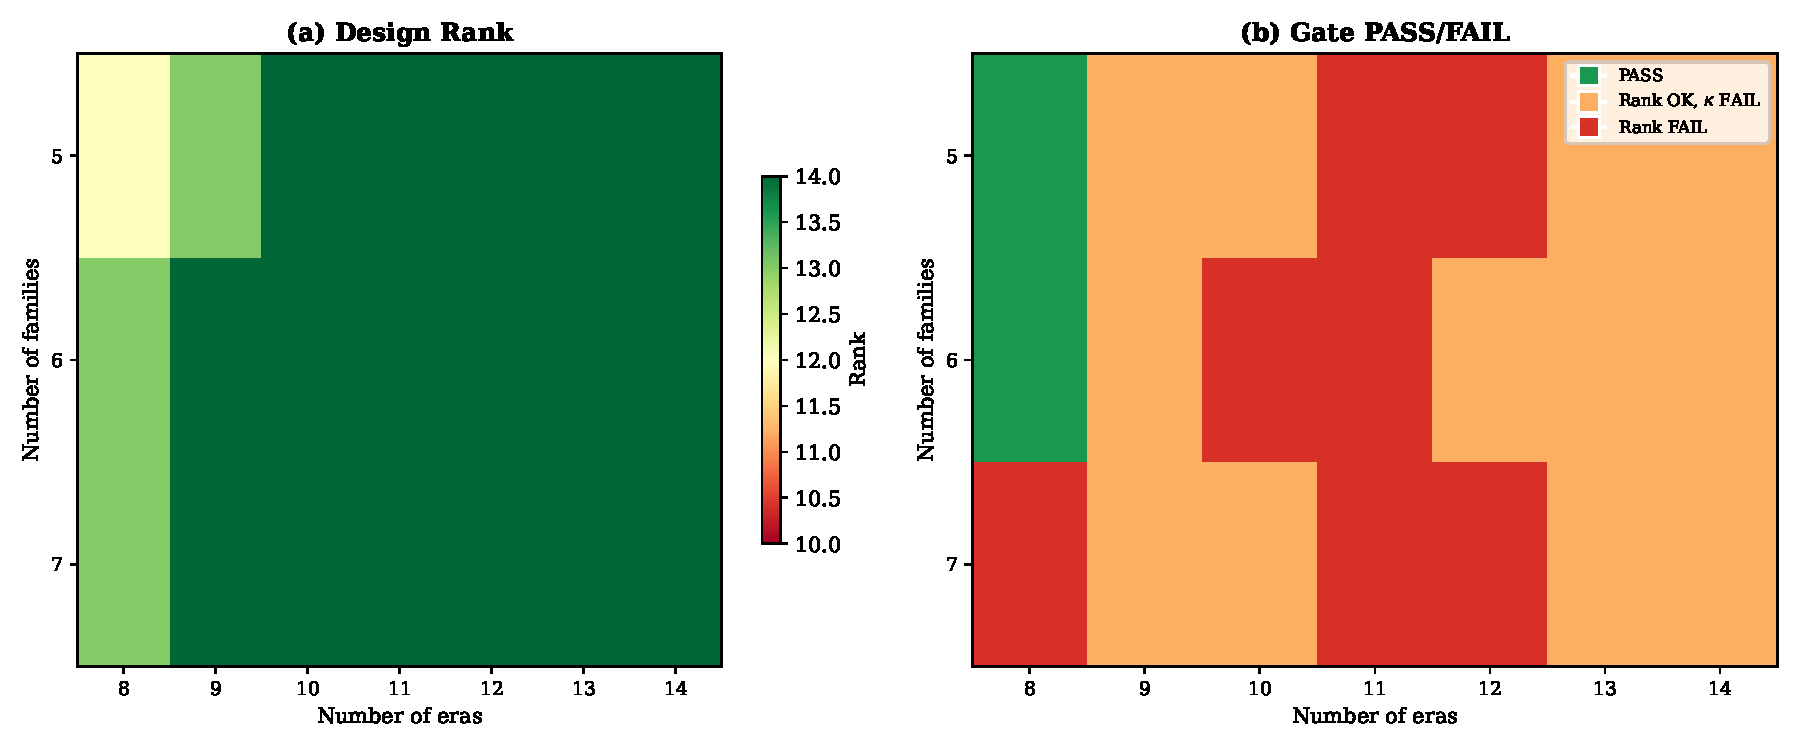
\includegraphics[width=\columnwidth]{fig8_design_heatmap.pdf}
\caption{\textbf{PASS/FAIL heatmap across the design space.} Each cell shows whether a given (N, F, E) configuration passes the three numerical/design-matrix diagnostics evaluated in the sweep: full rank, condition number, and VIF. Crossing and connectedness are enforced by the staggered assignment constraints. Within the evaluated configurations, passing designs cluster in regions with sufficient family and era representation.}
\label{fig:design_heatmap}
\end{figure}

\subsection{Outcome-Independent Selection Within the Candidate Frame}
The selection procedure (Algorithm~\ref{alg:g3}) selects the candidate subset from the 47-model candidate set. The structural minimum is 21 models (identifiable: full rank, VIF $\leq$ 10), but the 21-model design sits exactly on the recovery bar in simulation (era-share bias $\approx -5.0$pp with SE $0.6$--$0.8$pp---a knife-edge). Within the 47-model candidate frame, the selection procedure identifies a \textbf{22-model candidate subset} that clears the recovery bar at 300 repetitions (era bias A $+2.4$pp / B $-0.8$pp), passes the 1000-repetition margin confirmation (A $+2.2$pp / B $-2.4$pp), and is robust at 2000 repetitions (A $+1.7$pp / B $-3.2$pp). The extra model over the structural minimum is required by the pre-specified recovery criterion within this candidate frame. The 22-model population satisfies the structural gate conditions (S1--S3, N2) but does not satisfy the condition-number gate ($\kappa = 1100 > 100$); Algorithm~\ref{alg:g3} checks rank, VIF, and crossing but does not check $\kappa$, which is instead reported as a post-selection diagnostic. The 22-model subset is therefore not a fully gate-passing population; it is the outcome-independent candidate within this specific frame and under these specific selection criteria.

\subsection{Robustness and Sensitivity}
We characterize the sensitivity of the gate results to threshold choices and population perturbations.

\subsubsection{Condition-number threshold.} The baseline gate uses $\kappa_{\max} = 100$. At $\kappa_{\max} = 50$ the 16-model population still fails ($\kappa = 4.7 \times 10^{16}$), and the sufficient 30-model design still passes ($\kappa = 93$). At $\kappa_{\max} = 200$, the 6-family $\times$ 3-each design (18 models, rank 13/13, $\kappa = 164$) passes. The PASS/FAIL boundary is therefore robust across a factor-of-4 range in $\kappa_{\max}$.

\subsubsection{VIF threshold.} The baseline gate uses $\text{VIF}_{\max} = 10$. No design in the sweep passes all other gates while failing the VIF threshold, so the VIF gate is not the binding constraint for any evaluated configuration.

\subsubsection{Leave-one-model-out.} TABLE~\ref{tab:loo} reports structural diagnostics for each of the 16 leave-one-model-out configurations. Removing Llama-1 alone restores full rank (13/13) by eliminating the Llama family level and the 2023Q1 era level simultaneously. However, the resulting design does not satisfy the full identifiability gate: the condition number $\kappa = 585 > 100$, so the numerical stability criterion fails. All other removals leave the design rank-deficient with $\kappa \gg 10^{16}$. This demonstrates that rank deficiency and numerical instability are separable problems: fixing rank does not automatically fix conditioning.

\begin{table*}[!t]
\caption{\textbf{Leave-One-Model-Out Structural Diagnostics.} Removing Llama-1 restores full rank but does not satisfy the numerical stability gate ($\kappa = 585 > 100$). All other removals leave the design rank-deficient. The ``Binding'' column identifies which gate criterion remains unsatisfied after removal.}
\label{tab:loo}
\centering
\footnotesize
\begin{tabular}{l c c c c c l l}
\hline
\textbf{Removed} & \textbf{N} & \textbf{F} & \textbf{E} & \textbf{Rank} & $\boldsymbol{\kappa}$ & \textbf{Status} & \textbf{Binding} \\
\hline
Llama-1 & 15 & 4 & 10 & 13/13 & 585 & \textbf{FAIL} & $\kappa$ \\
\hline
Qwen-7B & 15 & 4 & 11 & 13/14 & $3.9\!\times\!10^{17}$ & FAIL & rank + $\kappa$ \\
\hline
Mistral-7B & 15 & 5 & 11 & 14/15 & $8.2\!\times\!10^{16}$ & FAIL & rank + $\kappa$ \\
\hline
Mistral-Small-3 & 15 & 5 & 11 & 14/15 & $4.9\!\times\!10^{16}$ & FAIL & rank + $\kappa$ \\
\hline
Mistral-Small-3.1 & 15 & 5 & 11 & 14/15 & $4.9\!\times\!10^{16}$ & FAIL & rank + $\kappa$ \\
\hline
Mistral-Small-3.2 & 15 & 5 & 11 & 14/15 & $6.2\!\times\!10^{16}$ & FAIL & rank + $\kappa$ \\
\hline
Devstral-2 & 15 & 5 & 10 & 13/14 & $6.7\!\times\!10^{16}$ & FAIL & rank + $\kappa$ \\
\hline
Mistral-Small-4 & 15 & 5 & 10 & 13/14 & $6.7\!\times\!10^{16}$ & FAIL & rank + $\kappa$ \\
\hline
Phi-1 & 15 & 5 & 10 & 13/14 & $2.0\!\times\!10^{17}$ & FAIL & rank + $\kappa$ \\
\hline
Phi-1.5 & 15 & 5 & 11 & 14/15 & $3.6\!\times\!10^{17}$ & FAIL & rank + $\kappa$ \\
\hline
Phi-2 & 15 & 5 & 10 & 13/14 & $1.6\!\times\!10^{17}$ & FAIL & rank + $\kappa$ \\
\hline
Phi-3 & 15 & 5 & 10 & 13/14 & $1.6\!\times\!10^{17}$ & FAIL & rank + $\kappa$ \\
\hline
Phi-4 & 15 & 5 & 10 & 13/14 & $1.6\!\times\!10^{17}$ & FAIL & rank + $\kappa$ \\
\hline
Phi-4-reas.+ & 15 & 5 & 11 & 14/15 & $1.1\!\times\!10^{17}$ & FAIL & rank + $\kappa$ \\
\hline
Gemma-3n & 15 & 5 & 11 & 13/15 & $5.2\!\times\!10^{17}$ & FAIL & rank + $\kappa$ \\
\hline
Gemma-4-12B & 15 & 5 & 10 & 13/14 & $3.2\!\times\!10^{17}$ & FAIL & rank + $\kappa$ \\
\hline
\end{tabular}
\end{table*}

\subsubsection{Era granularity.} TABLE~\ref{tab:era_res} reports gate diagnostics at three temporal resolutions. At quarter level (baseline), the design is rank-deficient with catastrophic conditioning ($\kappa = 4.7 \times 10^{16}$). Aggregating to half-year ($E = 7$ occupied levels) restores full rank (11/11) and improves conditioning to $\kappa = 227$, but the condition number still exceeds the $\kappa \leq 100$ threshold, so the numerical stability gate fails. Year-level aggregation ($E = 4$ occupied levels) also restores full rank (8/8) with $\kappa = 202 > 100$, again failing the numerical stability gate. The rank failure is specific to the quarterly resolution and is eliminated by coarser grouping. However, numerical instability persists at all three resolutions, demonstrating that rank deficiency and conditioning failure are separable problems.

\begin{table*}[!t]
\caption{\textbf{Era-Resolution Sensitivity.} Collapsing quarters to half-years or years eliminates rank deficiency but does not satisfy the full identifiability gate: $\kappa$ remains above the $\leq 100$ threshold at all resolutions.}
\label{tab:era_res}
\centering
\begin{tabular}{l c c c c c l l}
\hline
\textbf{Resolution} & \textbf{E} & \textbf{p} & \textbf{Rank} & $\boldsymbol{\kappa}$ & \textbf{VIF} & \textbf{Status} & \textbf{Binding} \\
\hline
Quarter (baseline) & 11 & 15 & 14/15 & $4.7\!\times\!10^{16}$ & $\infty$ & FAIL & rank + $\kappa$ + VIF \\
\hline
Half-year & 7 & 11 & 11/11 & 227 & 6.2 & FAIL & $\kappa$ \\
\hline
Year & 4 & 8 & 8/8 & 202 & 6.0 & FAIL & $\kappa$ \\
\hline
\end{tabular}
\end{table*}

\subsubsection{Contrast coding.} The baseline uses treatment (reference) coding. Sum-to-zero (deviation) coding produces rank 14/15, $\kappa = 3.6 \times 10^{16}$, VIF $= \infty$---the same FAIL verdict. The rank deficiency is structural (a consequence of the Llama--2023Q1 confound) and is not an artifact of the contrast parameterization.

\subsubsection{Fidelity sensitivity.} One model (Mistral-Small-4) was evaluated at 4-bit quantization rather than BF16. This does not affect the identifiability gate (which depends on design structure), but any future variance-component interpretation would need to account for the fidelity confound.

\section{Data Integrity, Threats to Validity, and Limitations}
\label{sec:threats}

\subsection{Data Integrity}
\begin{itemize}
\item The CSV aggregate accuracy values (TABLE~\ref{tab:accuracy}) are retained for descriptive and diagnostic analysis. The identifiability gate itself depends only on population structure and is independent of the observed trait values.
\item The per-question JSONL prediction files failed integrity validation: all 16 files contain constant predictions (every model predicts answer 0).
\item Model-by-item error-similarity analysis is therefore not reported and is deferred to future work once validated per-question prediction artifacts are available.
\item No model-by-item correlation claim is made from the empirical data.
\end{itemize}

\subsection{Internal Validity}
\begin{enumerate}
\item \textbf{Unverified evaluation validity.} Six models produce accuracy near the 4-choice chance level (23--25\%), and the Mistral-Small family shows a pronounced discontinuity between versions. The CSV values record artifact completeness, not necessarily evaluation validity. The identifiability gate result is invariant to the trait values, but any future variance-component interpretation requires independent validation of the accuracy measurements.
\item \textbf{Per-question JSONL integrity failure.} The JSONL artifacts are corrupted (constant predictions). Error-similarity analysis is deferred until validated per-question outputs are available.
\item \textbf{Mixed numerical fidelity.} One model (Mistral-Small-4) was evaluated at 4-bit quantization; all others at BF16. This introduces a confound between model identity and evaluation precision.
\end{enumerate}

\subsection{Construct Validity}
\begin{enumerate}
\item \textbf{Family $\neq$ true lineage.} The grouping factor ``family'' is a proxy for model lineage. True cross-generation lineage is largely undocumented in model cards; only 5 cross-generation edges are verified from metadata.
\item \textbf{Release quarter $\neq$ training era.} Release date is discretized to quarters, which simplifies temporal structure. Models released in the same quarter may have been trained on different data.
\item \textbf{MMLU accuracy $\neq$ overall capability.} The trait is measured on MMLU only; a benchmark weighted differently could yield different variance-component estimates.
\end{enumerate}

\subsection{Statistical Validity}
\begin{enumerate}
\item \textbf{Small $N$.} With only 16 models, the design is sparse and the family-era occupancy is incomplete.
\item \textbf{Sparse family-era occupancy.} 73\% of family-quarter cells are empty. Eight of 11 occupied quarters contain only one model.
\item \textbf{Threshold sensitivity.} The gate thresholds ($\kappa_{\max} = 100$, $\text{VIF}_{\max} = 10$) are conventional choices validated through simulation, not universal constants.
\item \textbf{Synthetic design assumptions.} The population-design analysis assumes a specific staggered assignment strategy. Other assignment strategies may yield different conditioning.
\item \textbf{Possible benchmark contamination.} If pretraining included MMLU items, trait variance is compressed toward zero and era/lineage shares are biased downward.
\end{enumerate}

\subsection{External Validity}
\begin{enumerate}
\item \textbf{Open-weight only.} Conclusions are scoped to the open-weight model population and do not generalize to closed or proprietary models.
\item \textbf{Single benchmark.} Results are scoped to MMLU 5-shot accuracy. Generalizability to other benchmarks is not established.
\item \textbf{No real population passes the full gate.} The sufficient configurations identified in Section~\ref{sec:sensitivity} are abstract population structures from a parameter sweep; we have not verified that a real set of currently available open-weight models instantiates this exact family-era distribution. The real-world outcome-independent candidate (22 models, from the actual 47-model pool) does not pass the full gate ($\kappa = 1100 > 100$). No population evaluated in this study---real or synthetic---both exists today and passes all five gate conditions simultaneously.
\end{enumerate}

\section{Discussion}
\label{sec:discussion}

\subsection{Main Methodological Finding}
The empirical analysis shows that variance decomposition of foundation-model performance requires pre-estimation identifiability checking, and that a realistic model population can fail those checks. Four of five gate conditions fail for the 16-model design; the 16-model design reflects the compute-feasible subset available in our study, not a deliberately pathological construction.

\subsection{What Was and Was Not Demonstrated}
The present study successfully demonstrates: (A) a formal identifiability framework for crossed variance-component models, (B) simulation-validated estimator behavior under identifiable and non-identifiable designs, (C) that the actual 16-model population fails the identifiability gate, and (D) a sufficient future population design through systematic design-space analysis. The study does not demonstrate: (E) actual family-proxy-vs-era variance shares (the gate failed), (F) empirical correlated-error structure (the JSONL data are corrupted), or (G) causal lineage effects (the observational design cannot support causal claims). The distinction between (A)--(D) and (E)--(G) should be kept clear throughout.

\subsection{Interpretation of the Negative Result}
The negative result---that the 16-model population fails the identifiability gate---is informative. It demonstrates that the gate works as designed: it catches a non-identifiable design before misleading inferences are reported. The 5.4\% family share is not a substantive finding; it is a diagnostic output of an invalid design. The CI covering $[0\%, 100\%]$ is the honest expression of that invalidity.

\subsection{Implications for Benchmark and Model-Panel Design}
\begin{itemize}
\item \textbf{For researchers:} Apply the identifiability gate before any variance decomposition of model populations. If the gate fails, the decomposition is not reportable regardless of what the estimator produces.
\item \textbf{For benchmark designers:} Ensure the evaluated model population spans enough families and eras with sufficient density.
\item \textbf{For the correlated-error literature:} Claims about whether diversifying across families reduces correlated error require a variance decomposition that is identifiable on the studied population.
\end{itemize}

\subsection{What Additional Empirical Data Would Be Needed}
To perform the intended family-proxy-era variance decomposition, a future study would need:
\begin{itemize}
\item A population satisfying comparable structural and recoverability criteria to the 22-model selection (full family-era crossing, adequate family count, sufficient density)
\item All 6 families represented with at least 2 models each
\item At least 8 occupied release quarters with at least 2 families per quarter (the sufficient designs explored here generally required this density under the evaluated staggered assignment strategy)
\item Validated per-question prediction data (not the corrupted JSONL artifacts available here)
\item Consistent numerical fidelity across all models
\end{itemize}

\section{Reproducibility and Open Science}
\label{sec:repro}

All analysis code, population definitions, simulation outputs, and design artifacts are available in the project repository.

\textbf{Environment:} Python 3.11.7, numpy 2.1.3, scipy 1.17.1, pandas 3.0.5, statsmodels 0.14.6, matplotlib 3.9.2.

\textbf{Key artifacts:}
\begin{itemize}
\item \texttt{datasets/phase2\_eval\_results.csv} --- 16-model empirical accuracy data (16-model aggregate evaluation artifacts; validity audit pending/ongoing)
\item \texttt{datasets/coverage/minimum\_valid\_population.csv} --- outcome-independent selected 22-model roster
\item \texttt{src/lineage\_era/analysis/reml.py} --- REML engine (CrossedREML, Woodbury-accelerated)
\item \texttt{src/lineage\_era/analysis/identifiability.py} --- Structural and fit-based audit gate
\item \texttt{src/lineage\_era/occupancy.py} --- 47-model population definition
\item \texttt{src/results/phase1/} --- D1/D2/D3/liability simulation outputs
\item \texttt{results/phase2\_empirical/audit\_summary.json} --- Gate diagnostic results
\end{itemize}

\textbf{Known invalid artifacts:}
\begin{itemize}
\item \texttt{datasets/eval\_samples/*.jsonl} --- All 16 files contain non-informative constant predictions (answer 0 for every question). NOT usable for per-question analysis.
\item \texttt{results/phase2\_empirical/similarity\_matrix\_phi.csv} --- All 1.0 (degenerate, from corrupted JSONL).
\item \texttt{results/phase2\_empirical/error\_matrix\_binary.csv} --- All 1s (from corrupted JSONL).
\end{itemize}

\textbf{Thresholds:} $\kappa_{\max} = 100$, $\text{VIF}_{\max} = 10$, $\text{BLUP}_{r} = 0.9$, $\text{SE}_{\text{inflation}} = 1.0$.

\textbf{Seeds:} Simulation uses recorded seeds per scenario (A=101, B=202, C=303).

\textbf{Verification note:} All numerical claims in the empirical identifiability results (rank, $\kappa$, VIF, occupancy, LOO diagnostics, diagnostic REML estimates) were independently verified by the authors against the source code and stored outputs. The design-space sweep results (105 evaluated configurations; 40 full rank; 3 $\kappa$-passing; 3 all-gate passing) and era-resolution half-year/year results were reproduced from the analysis scripts; the full per-configuration output is saved in \texttt{results/design\_space/sweep\_results.csv}.

\section{Conclusion}
\label{sec:conclusion}

We introduce an identifiability-gated framework for decomposing foundation-model performance into lineage, temporal, and model-specific components. The framework formalizes the structural and numerical conditions under which the decomposition is identifiable, and provides a pre-measurement gating procedure that detects failures before empirical inference is attempted.

The simulation study establishes that the direct REML estimator recovers known ground truth to within 2.5pp under balanced occupancy and 5.3pp under realistic sparse occupancy, and that three complementary detectors flag nested aliasing in 100\% of repetitions with zero silent coverage.

The empirical application to 16 real foundation models demonstrates that a realistic model population can fail the identifiability gate: the design is rank-deficient (rank 14 of 15), numerically unstable ($\kappa = 4.7 \times 10^{16}$), and has infinite variance inflation. Four of five gate conditions fail; only connectedness passes. The failure is structural, caused by a singleton family--era confound (Llama alone in 2023Q1) and additional crossing violations. The intended family-proxy-era variance decomposition is therefore not identifiable on this population and is not interpreted.

The population-design analysis identifies one sufficient configuration (30 models, 6 families, 8 eras) and characterizes the tradeoff between population size, family count, era count, and numerical conditioning. Within the evaluated 47-model candidate frame and the pre-specified selection criteria, the procedure selected a 22-model candidate subset; this design satisfies the structural gate (full rank, VIF $\leq$ 10, crossing) but not the condition-number gate ($\kappa = 1100 > 100$). The 22-model subset is therefore not a fully gate-passing population. Future studies would need a population satisfying comparable structural and recoverability criteria.

The main result is that the intended family-proxy-era attribution is not identifiable in the actual empirical population and that the proposed gate detects this before inference. The same design-gating principle may be applicable to other crossed random-effects analyses of model populations, and the gating procedure should be applied before any real-data variance-attribution claim.

\section*{Acknowledgment}
This work was supported in part by the Department of Computer Science and Engineering, SRM Institute of Science and Technology, Tiruchirappalli, India, and in part by the Research Institute of IoT Cybersecurity, National Kaohsiung University of Science and Technology, Kaohsiung, Taiwan.

\textbf{AI Disclosure:} AI language models were used during the preparation of this manuscript. Specific uses included: (1) code generation for simulation and analysis scripts, which was reviewed and verified by the authors; (2) figure layout and typesetting assistance; (3) manuscript formatting and language polishing. All scientific content, experimental design, data analysis, result interpretation, and conclusions were performed and verified entirely by the human authors. The authors take full responsibility for all content in this manuscript.

\begin{thebibliography}{35}

\bibitem{kim2025} E.~Kim, A.~Garg, K.~Peng, and N.~Garg, ``Correlated errors in
large language models,'' in \emph{Proc. Int. Conf. Mach. Learn. (ICML)},
vol.~267, pp.~30038--30066, 2025.

\bibitem{harville1977} D.~A.~Harville, ``Maximum likelihood approaches to variance
component estimation and to related problems,'' \emph{J. Amer. Statist. Assoc.},
vol.~72, no.~358, pp.~320--338, 1977.

\bibitem{patterson1971} H.~D.~Patterson and R.~Thompson, ``Recovery of
inter-block information when block sizes are unequal,'' \emph{Biometrika},
vol.~58, no.~3, pp.~545--554, 1971.

\bibitem{brennan2001} R.~L.~Brennan, \emph{Generalizability Theory}. New York, NY,
USA: Springer, 2001.

\bibitem{henderson1975} C.~R.~Henderson, ``Best linear unbiased estimation and
prediction under a selection model,'' \emph{Biometrics}, vol.~31, no.~2,
pp.~423--447, 1975.

\bibitem{searle1992} S.~R.~Searle, G.~Casella, and C.~E.~McCulloch,
\emph{Variance Components}. New York, NY, USA: Wiley, 1992.

\bibitem{rao1988} C.~R.~Rao and J.~Kleffe, \emph{Estimation of Variance
Components and Applications}. Amsterdam, The Netherlands: North-Holland, 1988.

\bibitem{mcculloch2001} C.~E.~McCulloch and S.~R.~Searle, \emph{Generalized,
Linear, and Mixed Models}. New York, NY, USA: Wiley, 2001.

\bibitem{laird1982} N.~M.~Laird and J.~H.~Ware, ``Random-effects models for
longitudinal data,'' \emph{Biometrics}, vol.~38, no.~4, pp.~963--974, 1982.

\bibitem{pinheiro2000} J.~C.~Pinheiro and D.~M.~Bates, \emph{Mixed-Effects
Models in S and S-PLUS}. New York, NY, USA: Springer, 2000.

\bibitem{bates2015} D.~Bates, M.~M\"{a}chler, B.~Bolker, and S.~Walker,
``Fitting linear mixed-effects models using lme4,'' \emph{J. Statist.
Software}, vol.~67, no.~1, pp.~1--48, 2015.

\bibitem{satterthwaite1946} F.~E.~Satterthwaite, ``An approximate distribution
of estimates of variance components,'' \emph{Biometrics Bull.}, vol.~2, no.~6,
pp.~110--114, 1946.

\bibitem{kenward1997} M.~G.~Kenward and J.~H.~Roger, ``Small sample inference
for fixed effects from restricted maximum likelihood,'' \emph{Biometrics},
vol.~53, no.~3, pp.~983--997, 1997.

\bibitem{cronbach1972} L.~J.~Cronbach, G.~C.~Gleser, H.~Nanda, and
N.~Rajaratnam, \emph{The Dependability of Behavioral Measurements}. New York, NY,
USA: Wiley, 1972.

\bibitem{snijders2012} T.~A.~B.~Snijders and R.~J.~Bosker, \emph{Multilevel
Analysis}, 2nd~ed. London, U.K.: Sage, 2012.

\bibitem{gelman2007} A.~Gelman and J.~Hill, \emph{Data Analysis Using Regression
and Multilevel/Hierarchical Models}. Cambridge, U.K.: Cambridge Univ. Press, 2007.

\bibitem{demidenko2013} E.~Demidenko, \emph{Mixed Models: Theory and Applications
with R}, 2nd~ed. Hoboken, NJ, USA: Wiley, 2013.

\bibitem{dietterich2000} T.~G.~Dietterich, ``Ensemble methods in machine
learning,'' in \emph{Proc. Int. Workshop Multiple Classifier Syst.}, LNCS 1857,
2000, pp.~1--15.

\bibitem{wolpert1992} D.~H.~Wolpert, ``Stacked generalization,'' \emph{Neural
Netw.}, vol.~5, no.~2, pp.~241--263, 1992.

\bibitem{breiman2001} L.~Breiman, ``Random forests,'' \emph{Mach. Learn.},
vol.~45, no.~1, pp.~5--38, 2001.

\bibitem{kuncheva2003} L.~I.~Kuncheva and C.~J.~Whitaker, ``Measures of
diversity in classifier ensembles and their relationship with the ensemble
accuracy,'' \emph{Mach. Learn.}, vol.~51, no.~2, pp.~181--207, 2003.

\bibitem{kleinberg2021} J.~Kleinberg and M.~Raghavan, ``Algorithmic monoculture
and social welfare,'' \emph{Proc. Nat. Acad. Sci. USA}, vol.~118, no.~22,
2021.

\bibitem{bommasani2022} R.~Bommasani, K.~A.~Creel, A.~Kumar, D.~Jurafsky, and
P.~Liang, ``Picking on the same person: Does algorithmic monoculture lead to
outcome homogenization?'' in \emph{Adv. Neural Inf. Process. Syst. (NeurIPS)},
vol.~35, 2022.

\bibitem{phylolm2024} N.~Yax, P.-Y.~Oudeyer, and S.~Palminteri, ``PhyloLM:
Inferring the phylogeny of large language models,'' in \emph{Proc. Int. Conf.
Learn. Represent. (ICLR)}, 2025.

\bibitem{jo2026} N.~Jo, N.~Garg, and M.~Raghavan, ``The subjectivity of
monoculture,'' 2026.

\bibitem{kuai2026} C.~Kuai \emph{et al.}, ``How independent are large language
models?'' 2026.

\bibitem{messing2026} S.~Messing, ``Decomposing and reducing hidden measurement
error in LLM evaluation pipelines,'' 2026.

\bibitem{li2026roots} Y.~Li \emph{et al.}, ``Tracing the roots,'' in \emph{Proc.
Annu. Meeting Assoc. Comput. Linguist. (ACL)}, 2026.

\bibitem{li2026pref} D.~Li \emph{et al.}, ``Preference leakage,'' in \emph{Proc.
Int. Conf. Learn. Represent. (ICLR)}, 2026.

\bibitem{hendrycks2021} D.~Hendrycks \emph{et al.}, ``Measuring massive multitask
language understanding,'' in \emph{Proc. Int. Conf. Learn. Represent. (ICLR)},
2021.

\bibitem{chen2026} J.~Chen, ``When does combining language models help?'' 2026.

\bibitem{self1987} S.~G.~Self and K.-Y.~Liang, ``Asymptotic properties of
maximum likelihood estimators and likelihood ratio tests under nonstandard
conditions,'' \emph{J. Amer. Statist. Assoc.}, vol.~82, no.~398, pp.~605--610,
1987.

\bibitem{stram1994} D.~O.~Stram and J.~W.~Lee, ``Variance components testing in
the longitudinal mixed effects model,'' \emph{Biometrics}, vol.~50, no.~4,
pp.~1171--1177, 1994.

\bibitem{efron1979} B.~Efron, ``Bootstrap methods: Another look at the
jackknife,'' \emph{Ann. Statist.}, vol.~7, no.~1, pp.~1--26, 1979.

\end{thebibliography}

\appendices

\section{Diagnostic Variance-Component Estimate}
\label{app:diagnostic}
Figure~\ref{fig:invalid} shows the diagnostic variance-component estimates obtained by fitting the family-share model to the non-identifiable 16-model design. The results are provided for completeness; the estimates are not scientifically interpretable.

\begin{figure}[H]
\centering
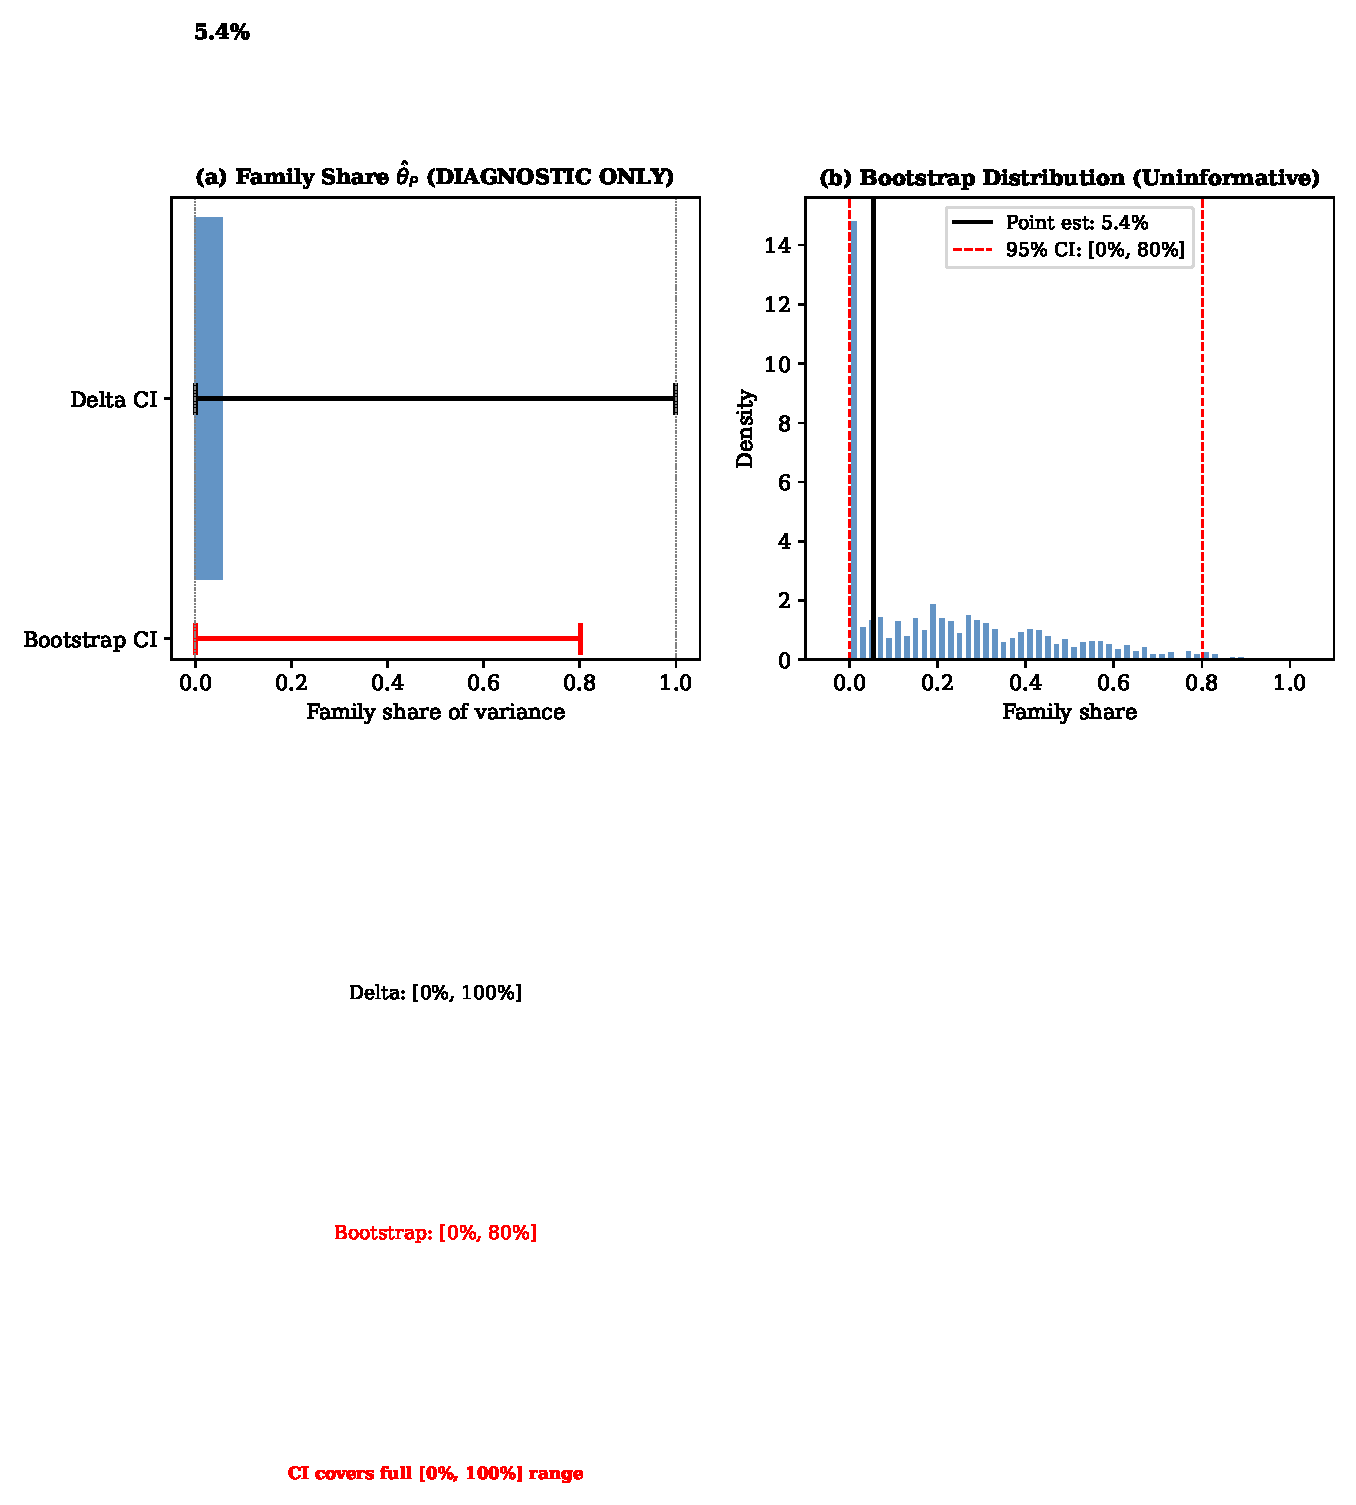
\includegraphics[width=\columnwidth]{fig6_invalid_design.pdf}
\caption{\textbf{Diagnostic variance-component estimates under the invalid (non-identifiable) 16-model design.} The 95\% confidence interval for the family share covers $[0\%, 100\%]$, reflecting the non-identifiability of the rank-deficient design. The near-zero era estimate is an aliasing artifact, not evidence of no era effect. This figure is provided for completeness; the estimates are not scientifically interpretable.}
\label{fig:invalid}
\end{figure}

\section{Outcome-Independent Candidate Population (22 Models)}
\label{app:22model}
TABLE~\ref{tab:22model} lists the 22 models selected by the outcome-independent procedure from the 47-model candidate population. The selection satisfies all structural gate conditions (S1--S3, N2) within the candidate frame, but does not satisfy the condition-number gate ($\kappa = 1100 > 100$) and is therefore not a fully gate-passing population.

\begin{table*}[!t]
\caption{\textbf{Outcome-Independent Candidate Population (22 Models).} Candidate subset from the 47-model frame, selected by the outcome-independent procedure. All 6 families are represented with $\geq 2$ models each. The selection crossing constraint requires every family to span $\geq 2$ eras and at least 2 eras to contain $\geq 2$ families; this subset satisfies both. This subset satisfies structural conditions (S1--S3, N2) but not the condition-number gate ($\kappa = 1100 > 100$).}
\label{tab:22model}
\centering
\footnotesize
\begin{tabular}{l l l c c c}
\hline
\textbf{Model} & \textbf{Family} & \textbf{Era} & \textbf{Params} & \textbf{Access} & \textbf{Measured?} \\
\hline
Llama-1 & Llama & 2023Q1 & 7B & Public & Yes \\
\hline
Llama-3.1-8B & Llama & 2024Q3 & 8B & Public & Yes \\
\hline
Llama-3.3-70B & Llama & 2024Q4 & 70B & Public & No \\
\hline
Qwen-7B & Qwen & 2023Q3 & 7B & Public & Yes \\
\hline
Qwen-1.5-72B & Qwen & 2024Q1 & 72B & Public & No \\
\hline
Mistral-7B & Mistral & 2023Q3 & 7B & Public & Yes \\
\hline
Mistral-Small-3 & Mistral & 2025Q1 & 24B & Public & Yes \\
\hline
Mistral-Small-3.1 & Mistral & 2025Q1 & 24B & Public & Yes \\
\hline
Mistral-Small-3.2 & Mistral & 2025Q2 & 24B & Public & Yes \\
\hline
Devstral-2 & Mistral & 2025Q4 & 24B & Public & Yes \\
\hline
Mistral-Small-4 & Mistral & 2026Q1 & 119B & Gated & Yes \\
\hline
Phi-1 & Phi & 2023Q2 & 1.3B & Public & Yes \\
\hline
Phi-1.5 & Phi & 2023Q3 & 1.3B & Public & Yes \\
\hline
Phi-2 & Phi & 2023Q4 & 2.7B & Public & Yes \\
\hline
Phi-3 & Phi & 2024Q2 & 14B & Public & Yes \\
\hline
Phi-4 & Phi & 2024Q4 & 14B & Public & Yes \\
\hline
Phi-4-reas.+ & Phi & 2025Q2 & 14B & Public & Yes \\
\hline
Phi-4-reas.-v. & Phi & 2026Q1 & 15B & Public & No \\
\hline
Gemma-3n & Gemma & 2025Q2 & 4B & Public & Yes \\
\hline
Gemma-4-12B & Gemma & 2026Q2 & 12B & Public & Yes \\
\hline
DeepSeek-V3.1 & DeepSeek & 2025Q3 & 685B & Public & No \\
\hline
DeepSeek-V3.2 & DeepSeek & 2025Q4 & 685B & Public & No \\
\hline
\end{tabular}
\end{table*}

\begin{IEEEbiographynophoto}{Sudharsan S}
received the B.E. degree in Computer Science and Engineering from the SRM Institute of Science and Technology, Tiruchirappalli, India, where he is currently pursuing the degree with the Department of Computer Science and Engineering. His research interests include natural language processing, large language model evaluation, and variance decomposition methods.
\end{IEEEbiographynophoto}

\begin{IEEEbiographynophoto}{S. Kanaga Suba Raja}
received the B.E. and M.E. degrees in Computer Science and Engineering. He is currently an Assistant Professor with the Department of Computer Science and Engineering, SRM Institute of Science and Technology, Tiruchirappalli, India, and a Visiting Researcher with the Research Institute of IoT Cybersecurity, National Kaohsiung University of Science and Technology, Kaohsiung, Taiwan. His research interests include machine learning, natural language processing, and statistical methods for AI evaluation.
\end{IEEEbiographynophoto}

\begin{IEEEbiographynophoto}{Shree Harish V}
received the degree from the SRM Institute of Science and Technology, Tiruchirappalli, India. He is currently with the Department of Computer Science and Engineering (Big Data Analytics), SRM Institute of Science and Technology, Tiruchirappalli, India. His research interests include cybersecurity, IoT, and AI systems.
\end{IEEEbiographynophoto}

\begin{IEEEbiographynophoto}{Chin-Shiuh Shieh}
received the Ph.D. degree in Electrical Engineering from National Cheng Kung University, Tainan, Taiwan. He is currently a Professor with the Department of Electrical Engineering, National Kaohsiung University of Science and Technology, Kaohsiung, Taiwan, and the Director of the Research Institute of IoT Cybersecurity. His research interests include wireless communications, signal processing, and IoT cybersecurity.
\end{IEEEbiographynophoto}

\begin{IEEEbiographynophoto}{Mong-Fong Horng}
received the Ph.D. degree in Electrical Engineering from National Cheng Kung University, Tainan, Taiwan. He is currently a Professor with the Department of Electrical Engineering, National Kaohsiung University of Science and Technology, Kaohsiung, Taiwan. His research interests include machine learning, data mining, and intelligent systems.
\end{IEEEbiographynophoto}

\begin{IEEEbiographynophoto}{Lavanya R}
received the degree from the SRM Institute of Science and Technology, Tiruchirappalli, India. She is currently with the Department of Computer Science and Engineering, SRM Institute of Science and Technology, Tiruchirappalli. Her research interests include machine learning and data analysis.
\end{IEEEbiographynophoto}

\EOD

\end{document}
